\PassOptionsToPackage{unicode=true}{hyperref} % options for packages loaded elsewhere
\PassOptionsToPackage{hyphens}{url}
%
\documentclass[]{book}
\usepackage{lmodern}
\usepackage{amssymb,amsmath}
\usepackage{ifxetex,ifluatex}
\usepackage{fixltx2e} % provides \textsubscript
\ifnum 0\ifxetex 1\fi\ifluatex 1\fi=0 % if pdftex
  \usepackage[T1]{fontenc}
  \usepackage[utf8]{inputenc}
  \usepackage{textcomp} % provides euro and other symbols
\else % if luatex or xelatex
  \usepackage{unicode-math}
  \defaultfontfeatures{Ligatures=TeX,Scale=MatchLowercase}
\fi
% use upquote if available, for straight quotes in verbatim environments
\IfFileExists{upquote.sty}{\usepackage{upquote}}{}
% use microtype if available
\IfFileExists{microtype.sty}{%
\usepackage[]{microtype}
\UseMicrotypeSet[protrusion]{basicmath} % disable protrusion for tt fonts
}{}
\IfFileExists{parskip.sty}{%
\usepackage{parskip}
}{% else
\setlength{\parindent}{0pt}
\setlength{\parskip}{6pt plus 2pt minus 1pt}
}
\usepackage{hyperref}
\hypersetup{
            pdftitle={Elements of Nonparametric Statistics},
            pdfauthor={Nicholas Henderson},
            pdfborder={0 0 0},
            breaklinks=true}
\urlstyle{same}  % don't use monospace font for urls
\usepackage{color}
\usepackage{fancyvrb}
\newcommand{\VerbBar}{|}
\newcommand{\VERB}{\Verb[commandchars=\\\{\}]}
\DefineVerbatimEnvironment{Highlighting}{Verbatim}{commandchars=\\\{\}}
% Add ',fontsize=\small' for more characters per line
\usepackage{framed}
\definecolor{shadecolor}{RGB}{248,248,248}
\newenvironment{Shaded}{\begin{snugshade}}{\end{snugshade}}
\newcommand{\AlertTok}[1]{\textcolor[rgb]{0.94,0.16,0.16}{#1}}
\newcommand{\AnnotationTok}[1]{\textcolor[rgb]{0.56,0.35,0.01}{\textbf{\textit{#1}}}}
\newcommand{\AttributeTok}[1]{\textcolor[rgb]{0.77,0.63,0.00}{#1}}
\newcommand{\BaseNTok}[1]{\textcolor[rgb]{0.00,0.00,0.81}{#1}}
\newcommand{\BuiltInTok}[1]{#1}
\newcommand{\CharTok}[1]{\textcolor[rgb]{0.31,0.60,0.02}{#1}}
\newcommand{\CommentTok}[1]{\textcolor[rgb]{0.56,0.35,0.01}{\textit{#1}}}
\newcommand{\CommentVarTok}[1]{\textcolor[rgb]{0.56,0.35,0.01}{\textbf{\textit{#1}}}}
\newcommand{\ConstantTok}[1]{\textcolor[rgb]{0.00,0.00,0.00}{#1}}
\newcommand{\ControlFlowTok}[1]{\textcolor[rgb]{0.13,0.29,0.53}{\textbf{#1}}}
\newcommand{\DataTypeTok}[1]{\textcolor[rgb]{0.13,0.29,0.53}{#1}}
\newcommand{\DecValTok}[1]{\textcolor[rgb]{0.00,0.00,0.81}{#1}}
\newcommand{\DocumentationTok}[1]{\textcolor[rgb]{0.56,0.35,0.01}{\textbf{\textit{#1}}}}
\newcommand{\ErrorTok}[1]{\textcolor[rgb]{0.64,0.00,0.00}{\textbf{#1}}}
\newcommand{\ExtensionTok}[1]{#1}
\newcommand{\FloatTok}[1]{\textcolor[rgb]{0.00,0.00,0.81}{#1}}
\newcommand{\FunctionTok}[1]{\textcolor[rgb]{0.00,0.00,0.00}{#1}}
\newcommand{\ImportTok}[1]{#1}
\newcommand{\InformationTok}[1]{\textcolor[rgb]{0.56,0.35,0.01}{\textbf{\textit{#1}}}}
\newcommand{\KeywordTok}[1]{\textcolor[rgb]{0.13,0.29,0.53}{\textbf{#1}}}
\newcommand{\NormalTok}[1]{#1}
\newcommand{\OperatorTok}[1]{\textcolor[rgb]{0.81,0.36,0.00}{\textbf{#1}}}
\newcommand{\OtherTok}[1]{\textcolor[rgb]{0.56,0.35,0.01}{#1}}
\newcommand{\PreprocessorTok}[1]{\textcolor[rgb]{0.56,0.35,0.01}{\textit{#1}}}
\newcommand{\RegionMarkerTok}[1]{#1}
\newcommand{\SpecialCharTok}[1]{\textcolor[rgb]{0.00,0.00,0.00}{#1}}
\newcommand{\SpecialStringTok}[1]{\textcolor[rgb]{0.31,0.60,0.02}{#1}}
\newcommand{\StringTok}[1]{\textcolor[rgb]{0.31,0.60,0.02}{#1}}
\newcommand{\VariableTok}[1]{\textcolor[rgb]{0.00,0.00,0.00}{#1}}
\newcommand{\VerbatimStringTok}[1]{\textcolor[rgb]{0.31,0.60,0.02}{#1}}
\newcommand{\WarningTok}[1]{\textcolor[rgb]{0.56,0.35,0.01}{\textbf{\textit{#1}}}}
\usepackage{longtable,booktabs}
% Fix footnotes in tables (requires footnote package)
\IfFileExists{footnote.sty}{\usepackage{footnote}\makesavenoteenv{longtable}}{}
\usepackage{graphicx,grffile}
\makeatletter
\def\maxwidth{\ifdim\Gin@nat@width>\linewidth\linewidth\else\Gin@nat@width\fi}
\def\maxheight{\ifdim\Gin@nat@height>\textheight\textheight\else\Gin@nat@height\fi}
\makeatother
% Scale images if necessary, so that they will not overflow the page
% margins by default, and it is still possible to overwrite the defaults
% using explicit options in \includegraphics[width, height, ...]{}
\setkeys{Gin}{width=\maxwidth,height=\maxheight,keepaspectratio}
\setlength{\emergencystretch}{3em}  % prevent overfull lines
\providecommand{\tightlist}{%
  \setlength{\itemsep}{0pt}\setlength{\parskip}{0pt}}
\setcounter{secnumdepth}{5}
% Redefines (sub)paragraphs to behave more like sections
\ifx\paragraph\undefined\else
\let\oldparagraph\paragraph
\renewcommand{\paragraph}[1]{\oldparagraph{#1}\mbox{}}
\fi
\ifx\subparagraph\undefined\else
\let\oldsubparagraph\subparagraph
\renewcommand{\subparagraph}[1]{\oldsubparagraph{#1}\mbox{}}
\fi

% set default figure placement to htbp
\makeatletter
\def\fps@figure{htbp}
\makeatother

\usepackage{booktabs}
\usepackage[]{natbib}
\bibliographystyle{apalike}

\title{Elements of Nonparametric Statistics}
\author{Nicholas Henderson}
\date{2020-01-26}

\begin{document}
\maketitle

{
\setcounter{tocdepth}{1}
\tableofcontents
}
\hypertarget{preface}{%
\chapter*{Preface}\label{preface}}
\addcontentsline{toc}{chapter}{Preface}

This book will serve as the main source of course notes for Biostatistics 685/Statistics 560, Winter 2020.

\hypertarget{intro}{%
\chapter{Introduction}\label{intro}}

\begin{center}\rule{0.5\linewidth}{\linethickness}\end{center}

\begin{center}\rule{0.5\linewidth}{\linethickness}\end{center}

\hypertarget{sec:whatisnonpar}{%
\section{What is Nonparametric Statistics?}\label{sec:whatisnonpar}}

\textbf{What is Parametric Statistics?}

\begin{itemize}
\item
  Parametric models refer to probability distributions that can
  be fully described by a fixed number of parameters that do not change
  with the sample size.
\item
  Typical examples include

  \begin{itemize}
  \tightlist
  \item
    Gaussian
  \item
    Poisson
  \item
    Exponential
  \item
    Beta
  \end{itemize}
\item
  Could also refer to a regression setting where the mean function
  is described by a fixed number of parameters.
\end{itemize}

\textbf{What is Nonparametric Statistics?}

\begin{itemize}
\item
  It is difficult to give a concise, all-encompassing definition, but nonparametric
  statistics generally refers to statistical methods where there is not a clear parametric component.
\item
  A more practical definition is that nonparametric statistics refers to flexible statistical procedures where
  very few assumptions are made regarding the distribution of the data or the form
  of a regression model.
\item
  The uses of nonparametric methods in several common statistical contexts are described in Sections \ref{sec:example-nonpar-tests} - \ref{sec:example-nonpar-regress2}.
\end{itemize}

\hypertarget{sec:course-outline}{%
\section{Outline of Course}\label{sec:course-outline}}

This course is roughly divided into the following 5 categories.

\begin{enumerate}
\def\labelenumi{\arabic{enumi}.}
\tightlist
\item
  \textbf{Nonparametric Testing}
\end{enumerate}

\begin{itemize}
\tightlist
\item
  Rank-based Tests
\item
  Permutation Tests
\end{itemize}

\begin{enumerate}
\def\labelenumi{\arabic{enumi}.}
\tightlist
\item
  \textbf{Estimation of Basic Nonparametric Quantities}
\end{enumerate}

\begin{itemize}
\tightlist
\item
  The Empirical Distribution Function
\item
  Density Estimation
\end{itemize}

\begin{enumerate}
\def\labelenumi{\arabic{enumi}.}
\tightlist
\item
  \textbf{Nonparametric Confidence Intervals}
\end{enumerate}

\begin{itemize}
\tightlist
\item
  Bootstrap
\item
  Jacknife
\end{itemize}

\begin{enumerate}
\def\labelenumi{\arabic{enumi}.}
\tightlist
\item
  \textbf{Nonparametric Regression Part I (Smoothing Methods)}
\end{enumerate}

\begin{itemize}
\tightlist
\item
  Kernel Methods
\item
  Splines
\item
  Local Regression
\end{itemize}

\begin{enumerate}
\def\labelenumi{\arabic{enumi}.}
\tightlist
\item
  \textbf{Nonparametric Regression Part II (Machine Learning Methods)}
\end{enumerate}

\begin{itemize}
\tightlist
\item
  Decision Trees/CART
\item
  Ensemble Methods
\end{itemize}

\hypertarget{sec:example-nonpar-tests}{%
\section{Example 1: Nonparametric vs.~Parametric Two-Sample Testing}\label{sec:example-nonpar-tests}}

Suppose we have data from two groups. For example, outcomes from
two different treatments.

\begin{itemize}
\item
  \textbf{Group 1 outcomes}: \(X_{1}, \ldots, X_{n}\) an i.i.d (independent and identically distributed) sample from distribution function \(F_{X}\).
  This means that
  \begin{equation}
  F_{X}(t) = P( X_{i} \leq t) \quad \textrm{ for any } 1 \leq i \leq n  \nonumber
  \end{equation}
\item
  \textbf{Group 2 outcomes}: \(Y_{1}, \ldots, Y_{m}\) an i.i.d. sample from distribution function \(F_{Y}\).
  \begin{equation}
  F_{Y}(t) = P( Y_{i} \leq t) \quad \textrm{ for any } 1 \leq i \leq n  \nonumber
  \end{equation}
\item
  To test the impact of a new treatment, we usually want to test whether or not \(F_{X}\) differs from \(F_{Y}\) in some way.
  This can be stated in hypothesis testing language as
  \begin{eqnarray}
  H_{0}&:& F_{X} = F_{Y} \quad \textrm{( populations are the same)} \nonumber \\
  H_{A}&:& F_{X} \neq F_{Y} \quad \textrm{( populations are different)} \label{eq:nonpar-twosample-hypothesis}
                                                                        \end{eqnarray}
\end{itemize}

\textbf{Parametric Tests}

\begin{itemize}
\item
  Perhaps the most common parametric test for \eqref{eq:nonpar-twosample-hypothesis} is the \textbf{t-test}. The t-test assumes that
  \begin{equation}
  F_{X} = \textrm{Normal}(\mu_{x}, \sigma^{2}) \quad \textrm{ and } \quad F_{Y} = \textrm{Normal}(\mu_{y}, \sigma^{2})
  \end{equation}
\item
  Under this parametric assumption, the hypothesis test \eqref{eq:nonpar-twosample-hypothesis} reduces to
  \begin{equation}
  H_{0}: \mu_{x} = \mu_{y}  \quad \textrm{ vs. } \quad H_{A}: \mu_{x} \neq \mu_{y}
  \end{equation}
\item
  The standard t-statistic (with a pooled estimate of \(\sigma^{2}\)) is the following
  \begin{equation}
  T = \frac{\bar{X} - \bar{Y}}{ s_{p}\sqrt{\frac{1}{n} + \frac{1}{m}}  },
  \end{equation}
  where \(\bar{X} = \frac{1}{n}\sum_{i=1}^{n} X_{i}\) and \(\bar{Y} = \frac{1}{m}\sum_{i=1}^{m} Y_{i}\) are
  the group-specific sample means and \(s_{p}^{2}\) is the pooled estimate of \(\sigma^{2}\)
  \begin{equation}
  s_{p}^{2} = \frac{1}{m + n - 2}\Big\{ \sum_{i=1}^{n} (X_{i} - \bar{X})^{2} + \sum_{i=1}^{m} (Y_{i} - \bar{Y})^{2}   \Big\}
  \end{equation}
\end{itemize}

\begin{center}\rule{0.5\linewidth}{\linethickness}\end{center}

\begin{itemize}
\item
  The t-test is based on the \textbf{null distribution} of \(T\) - the distribution of \(T\) under the null hypothesis.
\item
  Under the assumption of normality, the null distribution of \(T\) is a t distribution with \(n + m - 2\) degrees of freedom.
\end{itemize}

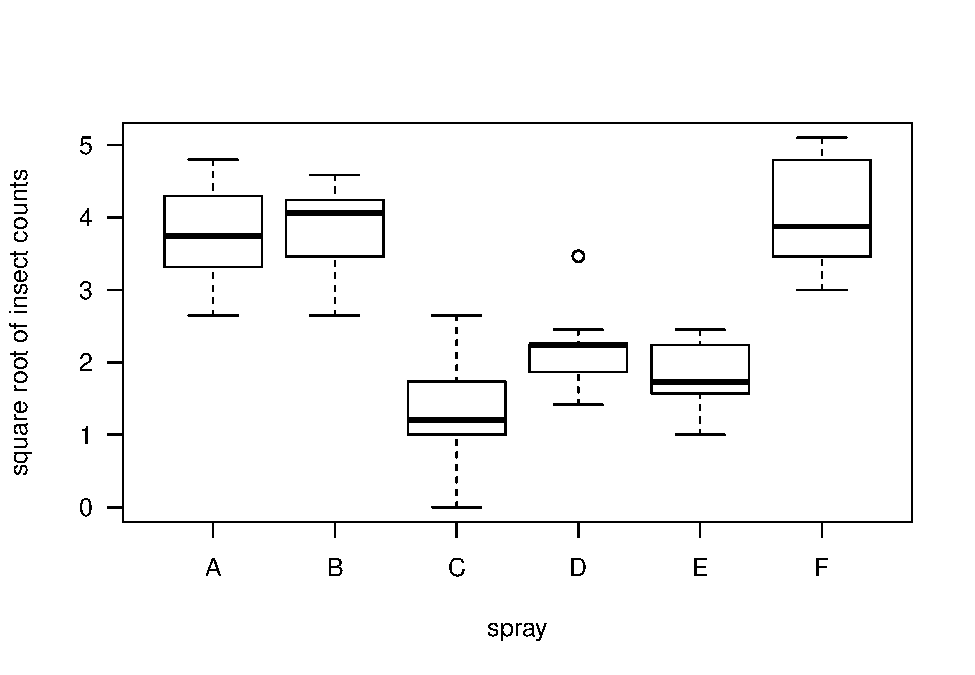
\includegraphics{01-IntroductionLatex_files/figure-latex/unnamed-chunk-2-1.pdf}

\begin{itemize}
\item
  Notice that the null distribution of \(T\) depends on the parametric assumption that both \(F_{X} = \textrm{Normal}(\mu_{x}, \sigma^{2})\)
  and \(F_{Y} = \textrm{Normal}(\mu_{y}, \sigma^{2})\). Appealing to the Central Limit Theorem, one could
  argue that is a quite reasonable assumption.
\item
  In addition to using the assumption that \(F_{X} = \textrm{Normal}(\mu_{x}, \sigma^{2})\) and \(F_{Y} = \textrm{Normal}(\mu_{y}, \sigma^{2})\), we used this parametric assumption (at least implicitly) in the formulation of the hypothesis test itself because we assumed that any difference between \(F_{X}\) and \(F_{Y}\) would be fully described by difference in \(\mu_{x}\) and \(\mu_{y}\).
\item
  So, in a sense, you are using the assumption of normality twice in the construction of the two-sample t-test.
\end{itemize}

\begin{center}\rule{0.5\linewidth}{\linethickness}\end{center}

\textbf{Nonparametric Tests}

\begin{itemize}
\item
  Two-sample nonparametric tests are meant to be ``distribution-free''. This means the null distribution of the test statistic does not depend on any parametric
  assumptions about the two populations \(F_{X}\) and \(F_{Y}\).
\item
  Many such tests are based on \textbf{ranks}. The distribution of the ranks under the assumption that \(F_{X} = F_{Y}\) do
  not depend on the form of \(F_{X}\) (assuming \(F_{X}\) is continuous).
\item
  Also, the statements of hypotheses tests for nonparametric tests should not rely on any parametric assumptions about \(F_{X}\) and \(F_{Y}\).
\item
  For example, \(H_{A}: F_{X} \neq F_{Y}\) or \(H_{A}: F_{X} \geq F_{Y}\).
\end{itemize}

\begin{center}\rule{0.5\linewidth}{\linethickness}\end{center}

\begin{itemize}
\item
  Nonparametric tests usually tradeoff power for greater robustness.
\item
  In general, if the parametric assumptions are correct, a nonparametric test will have less power than its parametric counterpart.
\item
  If the parametric assumptions are not correct, parametric tests might have inappropriate type-I error control
  or lose power.
\end{itemize}

\hypertarget{sec:example-nonpar-estimation}{%
\section{Example 2: Nonparametric Estimation}\label{sec:example-nonpar-estimation}}

\begin{itemize}
\item
  Suppose we have \(n\) observations \((X_{1}, \ldots, X_{n})\) which are assumed to be i.i.d. (independent and identically distributed).
  The distribution function of \(X_{i}\) is \(F_{X}\).
\item
  Suppose we are interested in estimating the entire distribution function \(F_{X}\) rather than specific features
  of the distribution of \(X_{i}\) such as the mean or standard deviation.
\item
  In a \textbf{parametric} approach to estimating \(F_{X}\), we would assume the distribution of \(X_{i}\) belongs to some parametric family of distributions.
  For example,

  \begin{itemize}
  \tightlist
  \item
    \(X_{i} \sim \textrm{Normal}(\mu, \sigma^{2})\)
  \item
    \(X_{i} \sim \textrm{Exponential}(\lambda)\)
  \item
    \(X_{i} \sim \textrm{Beta}(\alpha, \beta)\)
  \end{itemize}
\end{itemize}

\begin{center}\rule{0.5\linewidth}{\linethickness}\end{center}

\begin{itemize}
\item
  If we assume that \(X_{i} \sim \textrm{Normal}( \mu, \sigma^{2} )\), we only need to estimate 2 parameters to
  fully describe the distribution of \(X_{i}\), and the number of parameters will not depend on the sample size.
\item
  In a nonparametric approach to characterizing the distribution of \(X_{i}\), we need to instead
  estimate the entire distribution function \(F_{X}\) or density function \(f_{X}\).
\item
  The distribution function \(F_{X}\) is usually estimated by the \textbf{empirical distribution function}
  \begin{equation}
  \hat{F}_{n}(t) = \frac{1}{n}\sum_{i=1}^{n} I( X_{i} \leq t),
  \end{equation}
  where \(I()\) denotes the indicator function. That is, \(I( X_{i} \leq t) = 1\) if \(X_{i} \leq t\),
  and \(I(X_{i} \leq t) = 0\) if \(X_{i} > t\).
\item
  The empirical distribution function is a discrete distribution function,
  and it can be thought of as an estimate having \(n\) "parameters.
\item
  The density function of \(X_{i}\) is often estimated by a kernel density estimator (KDE). This
  is defined as
  \begin{equation}
  \hat{f}_{n}(t) = \frac{1}{n h_{n}} \sum_{i=1}^{n} K\Big( \frac{t - X_{i}}{ h_{n} } \Big).
  \end{equation}
\item
  \(K()\) - the kernel function
\item
  \(h_{n}\) - the bandwidth
\item
  The KDE is a type of smoothing procedure.
\end{itemize}

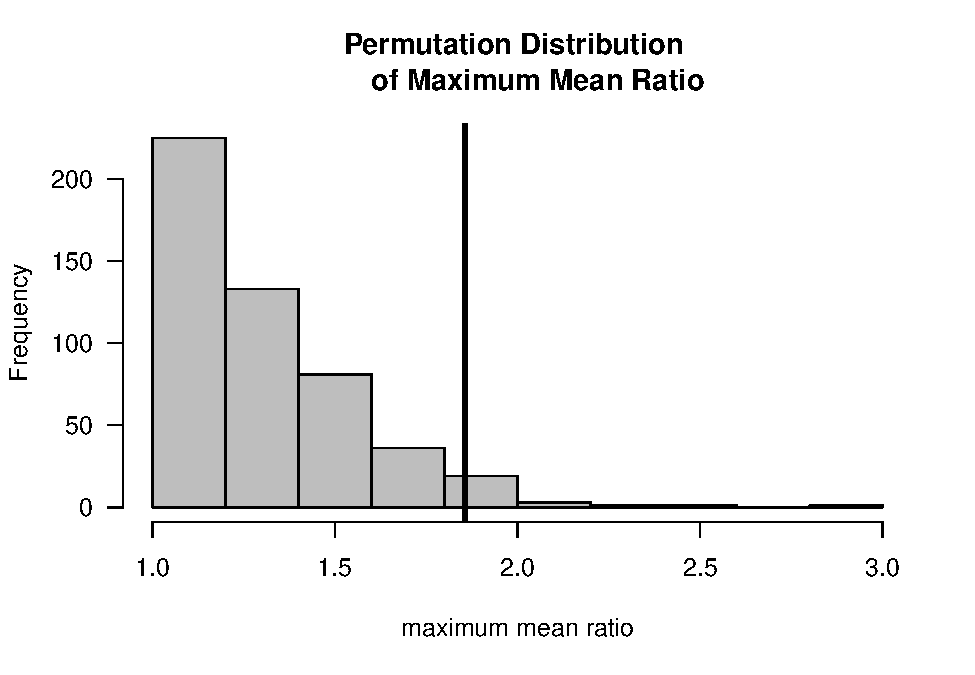
\includegraphics{01-IntroductionLatex_files/figure-latex/unnamed-chunk-3-1.pdf} 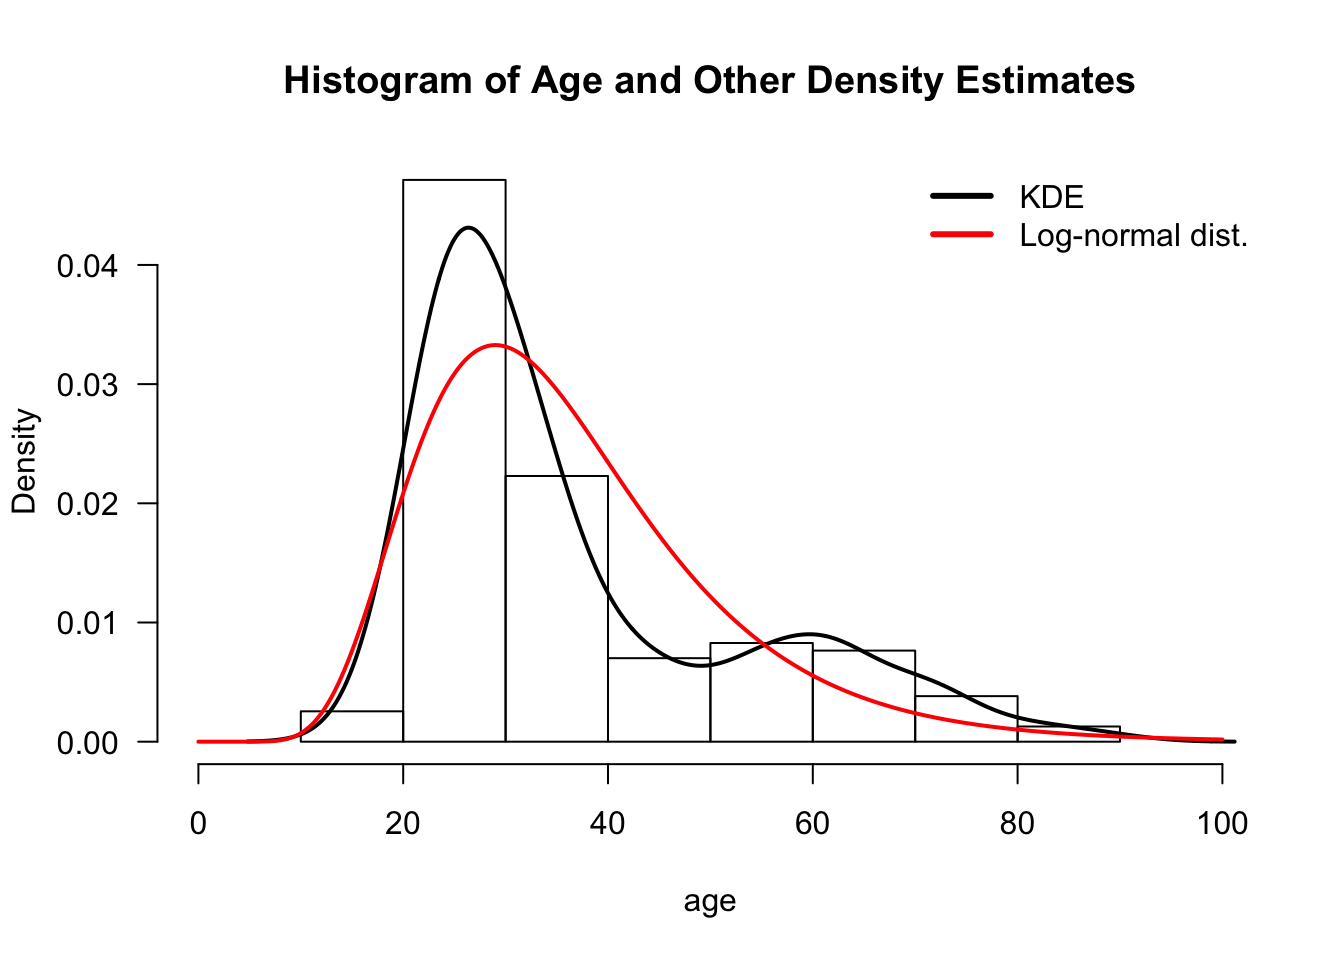
\includegraphics{01-IntroductionLatex_files/figure-latex/unnamed-chunk-3-2.pdf}

\hypertarget{sec:example-nonpar-confint}{%
\section{Example 3: Confidence Intervals}\label{sec:example-nonpar-confint}}

\begin{itemize}
\item
  Inference for a wide range of statistical procedures is based on the following argument
  \begin{equation}
  \hat{\theta}_{n} \textrm{ has an approximate Normal}\Big( \theta, \widehat{\textrm{Var}(\hat{\theta}_{n})} \Big) \textrm{ distribution }
  \label{eq:normal-approx}
  \end{equation}
\item
  Above, \(\hat{\theta}_{n}\) is an estimate of a parameter \(\theta\), and \(\widehat{\textrm{Var}(\hat{\theta}_{n})}\) is an estimate of the variance of \(\hat{\theta}_{n}\).
\item
  \(se_{n} = \sqrt{\widehat{\textrm{Var}(\hat{\theta}_{n})}}\) is usually referred to as the \textbf{standard error}.
\item
  \(95\%\) confidence intervals are reported using the following formula
  \begin{equation}
  [\hat{\theta}_{n} - 1.96 se_{n}, \hat{\theta}_{n} + 1.96 se_{n}  ]
  \end{equation}
\item
  Common examples of this include:

  \begin{enumerate}
  \def\labelenumi{\arabic{enumi}.}
  \tightlist
  \item
    \(\hat{\theta}_{n} = \bar{X}_{n}\).
  \end{enumerate}

  In this case, appeals to the Central Limit Theorem would justify approximation \eqref{eq:normal-approx}. The variance of \(\hat{\theta}_{n}\) would be \(\sigma^{2}\), and the standard error would typically be \(se_{n} = \hat{\sigma}/\sqrt{n}\).

  \begin{enumerate}
  \def\labelenumi{\arabic{enumi}.}
  \setcounter{enumi}{1}
  \tightlist
  \item
    \(\hat{\theta}_{n} = \textrm{Maximum Likelihood Estimate of } \theta\).
  \end{enumerate}

  In this case, asymptotics would justify the approximate distribution \(\hat{\theta}_{n} \sim \textrm{Normal}(\theta, \frac{1}{nI(\theta)} )\), where \(I(\theta)\) denotes the Fisher information. The standard error in this context is often \(se_{n} = \{ n I(\hat{\theta}_{n}) \}^{-1/2}\).
\end{itemize}

\begin{center}\rule{0.5\linewidth}{\linethickness}\end{center}

\begin{itemize}
\item
  Confidence intervals using \eqref{eq:normal-approx} rely on a parametric approximation to the
  sampling distribution of the statistic \(\hat{\theta}_{n}\).
\item
  Moreover, even if one wanted to use something like \eqref{eq:normal-approx}, working out
  standard error formulas can be a great challenge in more complicated situations.
\end{itemize}

\begin{center}\rule{0.5\linewidth}{\linethickness}\end{center}

\begin{itemize}
\item
  The \textbf{bootstrap} is a simulation-based approach for computing standard errors and
  confidence intervals.
\item
  The bootstrap does not rely on any particular parametric assumptions and
  can be applied in almost any context
  (though bootstrap confidence intervals can fail to work as desired in some situations).
\item
  Through resampling from the original dataset, the bootstrap uses many possible alternative datasets to
  assess the variability in \(\hat{\theta}_{n}\).
\end{itemize}

\begin{table}[ht]
\centering
\begin{tabular}{cccccc}
  \hline
 & OriginalDat & Dat1 & Dat2 & Dat3 & Dat4 \\ 
  \hline
Obs. 1 & 0.20 & 0.20 & 0.80 & 0.20 & 0.30 \\ 
  Obs. 2 & 0.50 & 0.20 & 0.80 & 0.20 & 0.70 \\ 
  Obs. 3 & 0.30 & 0.30 & 0.50 & 0.80 & 0.20 \\ 
  Obs. 4 & 0.80 & 0.30 & 0.70 & 0.50 & 0.50 \\ 
  Obs. 5 & 0.70 & 0.70 & 0.20 & 0.30 & 0.20 \\ 
  theta.hat & 0.50 & 0.34 & 0.60 & 0.40 & 0.38 \\ 
   \hline
\end{tabular}
\end{table}

\begin{center}\rule{0.5\linewidth}{\linethickness}\end{center}

\begin{itemize}
\item
  In the above example, we have 4 \textbf{boostrap replications} for the statistic \(\hat{\theta}\):
  \begin{eqnarray}
  \hat{\theta}^{(1)} &=& 0.34 \\ 
  \hat{\theta}^{(2)} &=& 0.60 \\
  \hat{\theta}^{(3)} &=& 0.40 \\ 
  \hat{\theta}^{(4)} &=& 0.38
  \end{eqnarray}
\item
  In the above example, the bootstrap standard error for \(\hat{\theta}_{n}\) would be
  the standard deviation of the bootstrap replications
  \begin{eqnarray}
  se_{boot} &=& \Big( \frac{1}{3} \sum_{b=1}^{4} \{ \hat{\theta}^{(b)} - \hat{\theta}^{(-)}  \}^{2} \Big)^{1/2} \nonumber \\
  &=& \Big( (0.34 - 0.43)^{2}/3 + (0.60 - 0.43)^{2}/3 + (0.40 - 0.43)^{2}/3 + (0.38 - 0.43)^{2}/3 \Big)^{1/2} \nonumber \\
  &=& 0.116
  \end{eqnarray}
  where \(\hat{\theta}^{(-)} = 0.43\) is the average of the bootstrap replications.
\item
  One would then report the confidence interval \([\hat{\theta} - 1.96 \times 0.116, \hat{\theta} + 1.96 \times 0.116]\).
  In practice, the number of bootstrap replications is typically much larger than \(4\).
\item
  It is often better to construct confidence intervals using the percentiles from the bootstrap distribution
  of \(\hat{\theta}\) rather than use a confidence interval of the form: \(\hat{\theta} \pm 1.96 \times se_{boot}\).
\end{itemize}

\begin{figure}
\centering
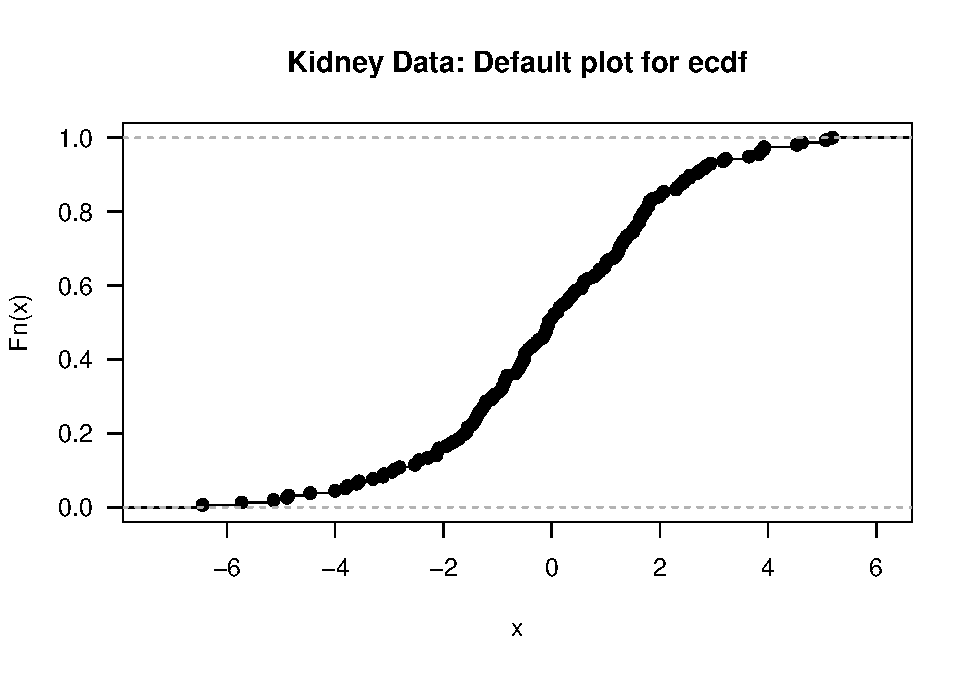
\includegraphics{01-IntroductionLatex_files/figure-latex/unnamed-chunk-4-1.pdf}
\caption{\label{fig:unnamed-chunk-4}Bootstrap distribution of the sample standard deviation for the age variable from the kidney fitness data. Dasjed vertical lines are placed at the 2.5 and 97.5 percentiles of the bootstrap distribution.}
\end{figure}

\hypertarget{sec:example-nonpar-regress1}{%
\section{Example 4: Nonparametric Regression with a Single Covariate}\label{sec:example-nonpar-regress1}}

\begin{itemize}
\item
  Regression is a common way of modeling the relationship between two different variables.
\item
  Suppose we have \(n\) pairs of observations \((y_{1}, x_{1}), \ldots, (y_{n}, x_{n})\) where
  \(y_{i}\) and \(x_{i}\) are suspected to have some association.
\item
  Linear regression would assume that these \(y_{i}\) and \(x_{i}\) are related by the following
  \begin{equation}
  y_{i} = \beta_{0} + \beta_{1}x_{i} + \varepsilon_{i} 
  \end{equation}
  with the assumption \(\varepsilon_{i} \sim \textrm{Normal}(0, \sigma^{2})\) often made.
\item
  In this model, there are only 3 parameters: \((\beta_{0}, \beta_{1}, \sigma^{2})\),
  and the number of parameters stays fixed for all \(n\).
\end{itemize}

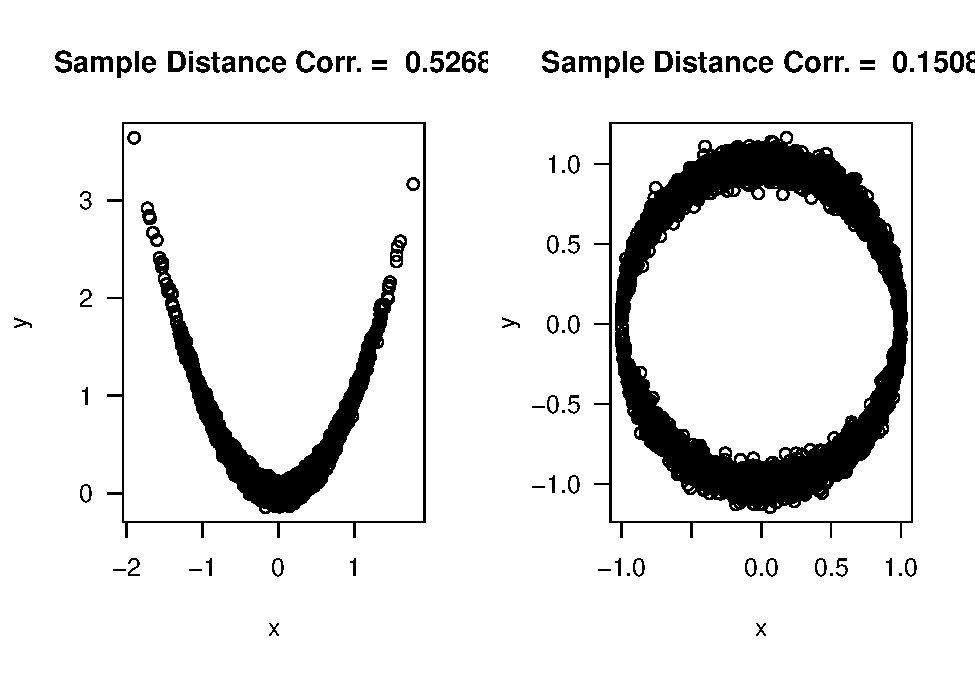
\includegraphics{01-IntroductionLatex_files/figure-latex/unnamed-chunk-5-1.pdf}

\begin{center}\rule{0.5\linewidth}{\linethickness}\end{center}

\begin{itemize}
\item
  The nonparametric counterpart to linear regression is usually formulated in the following way
  \begin{equation}
  y_{i} = m( x_{i} ) + \varepsilon_{i}
  \end{equation}
\item
  Typically, one makes very few assumptions about the form of the mean function \(m\), and it is not assumed \(m\)
  can be described by a finite number of parameters.
\item
  There are a large number of nonparametric methods for estimating \(m\).
\item
  One popular method is the use of \textbf{smoothing splines}.
\item
  With smoothing splines, one considers mean functions of the form
  \begin{equation}
  m(x) = \sum_{j=1}^{n} \beta_{j}g_{j}(x) 
  \label{eq:smoothspline-model}
  \end{equation}
  where \(g_{1}, \ldots, g_{n}(x)\) are a collection of spline basis functions.
\end{itemize}

\begin{center}\rule{0.5\linewidth}{\linethickness}\end{center}

\begin{itemize}
\item
  Because of the large number of parameters in \eqref{eq:smoothspline-model}, one should
  estimate the basis function weights \(\beta_{j}\) through penalized regression
  \begin{equation}
  \textrm{minimize} \quad \sum_{i=1}^{n} \Big( y_{i} - \sum_{j=1}^{n} \beta_{j}g_{j}( x_{i} ) \Big)^{2} + \lambda \sum_{i=1}^{n}\sum_{j=1}^{n} \Omega_{ij}\beta_{i}\beta_{j}
  \label{eq:smoothspline-estimation}
  \end{equation}
  where \(\Omega_{ij} = \int g_{i}''(t)g_{j}''(t) dt\).
\item
  Using coefficient estimates \(\hat{\beta}_{1}, \ldots, \hat{\beta}_{n}\) found from solving \eqref{eq:smoothspline-model}, the nonparametric estimate of the mean function is defined as
  \begin{equation}
  \hat{m}(x) = \sum_{j=1}^{n} \hat{\beta}_{j}g_{j}(x) 
  \end{equation}
\item
  While the estimation in \eqref{eq:smoothspline-estimation} resembles parametric estimation for linear regression, notice
  that the number of parameters to be estimated will change with the sample size.
\item
  Allowing the number of basis functions to grow with \(n\) is important. For a sufficiently large number of basis functions, one should be able to approximate the
  true mean function \(m(x)\) arbitrarily closely.
\end{itemize}

\includegraphics{01-IntroductionLatex_files/figure-latex/unnamed-chunk-6-1.pdf}

\hypertarget{sec:example-nonpar-regress2}{%
\section{Example 5: Classification and Regression Trees (CART)}\label{sec:example-nonpar-regress2}}

\begin{itemize}
\item
  Suppose we now have observations \((y_{1}, \mathbf{x}_{1}), \ldots, (y_{n}, \mathbf{x}_{n})\) where
  \(y_{i}\) is a continuous response and \(\mathbf{x}_{i}\) is a p-dimensional vector of covariates.
\item
  Regression trees are a nonparametric approach for predicting \(y_{i}\) from \(\mathbf{x}_{i}\).
\item
  Here, the regression function is a \textbf{decision tree} rather than some fitted curve.
\item
  With a decision tree, a final prediction from a covariate vector \(\mathbf{x}_{i}\) is obtained by answering
  a sequence of ``yes or no'' questions.
\item
  When the responses \(y_{i}\) are binary, such trees are referred to as classification trees.
  Hence, the name: classification and regression trees (CART).
\end{itemize}

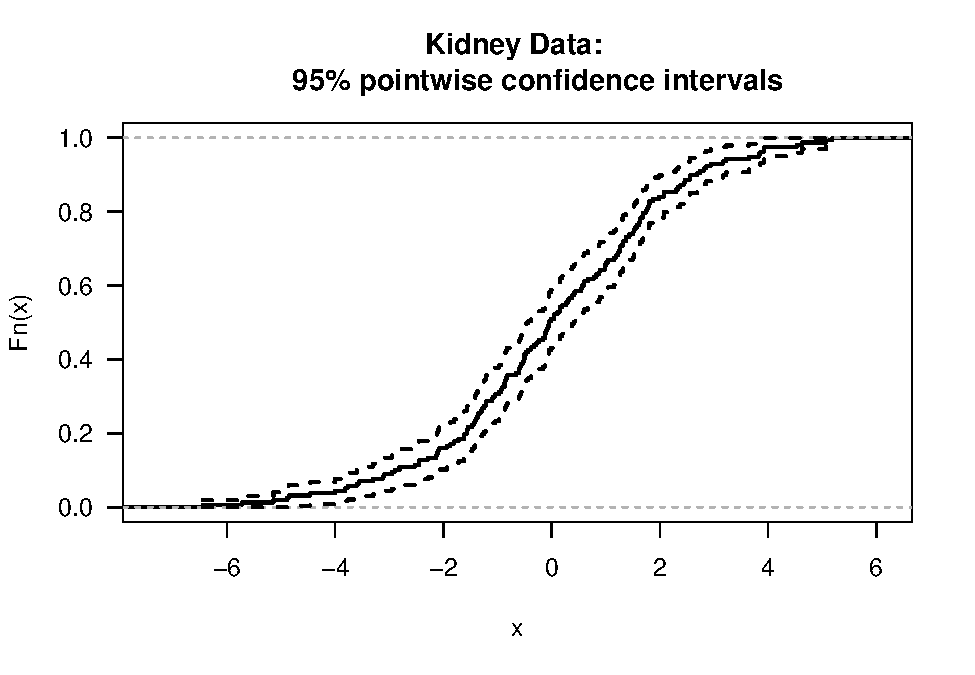
\includegraphics{01-IntroductionLatex_files/figure-latex/unnamed-chunk-7-1.pdf}

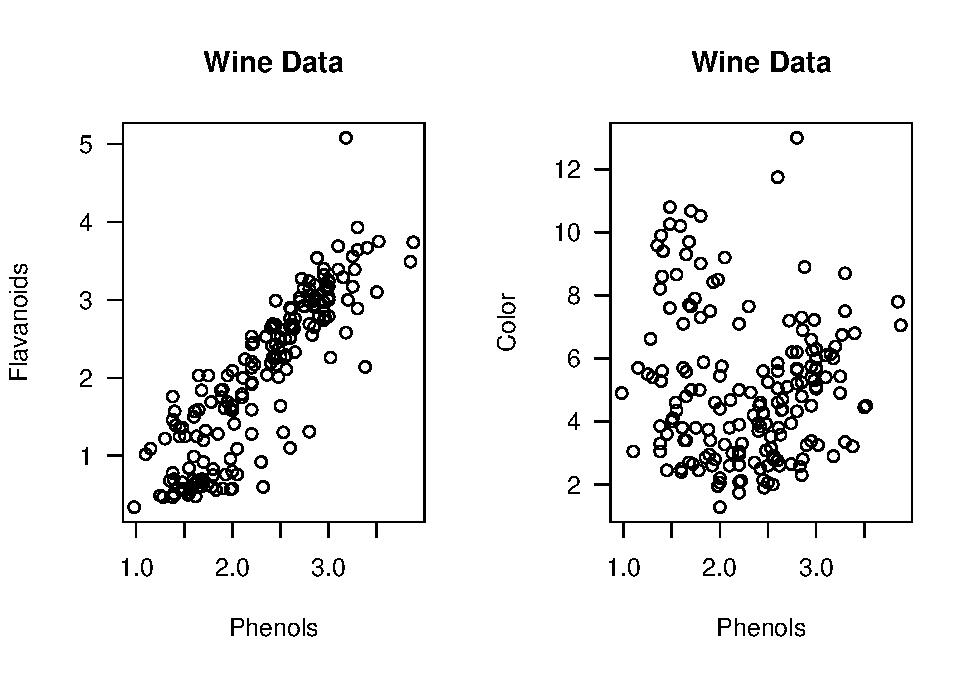
\includegraphics{01-IntroductionLatex_files/figure-latex/unnamed-chunk-8-1.pdf}

\begin{center}\rule{0.5\linewidth}{\linethickness}\end{center}

\begin{itemize}
\item
  Classification and regression trees are constructed through \textbf{recursive partitioning}.
\item
  Recursive partitioning is the process of deciding if and how to split a given
  node into two child nodes.
\item
  Tree splits are usually chosen to minimize the ``within-node'' sum of squares.
\item
  The size of the final is determined by a process of ``pruning'' the tree
  with cross-validation determining the best place to stop pruning.
\item
  Regression trees are an example of a more algorithmic approach to
  constructing predictions (as opposed to probability modeling in more
  traditional statistical methods) with a strong emphasis on predictive
  performance as measured through cross-validation.
\end{itemize}

\begin{center}\rule{0.5\linewidth}{\linethickness}\end{center}

\begin{itemize}
\item
  While single regression trees have the advantage of being directly interpretable,
  their prediction performance is often not that great.
\item
  However, using collections of trees can be very effective for prediction and
  has been used in many popular learning methods. Examples include: random forests,
  boosting, and Bayesian additive regression trees (BART).
\item
  Methods such as these can perform well on much larger datasets. We will discuss
  additional methods if time allows.
\end{itemize}

\hypertarget{getting-started}{%
\chapter{Working with R}\label{getting-started}}

You can download R by visiting \url{https://www.r-project.org/} and clicking on the \textbf{download R} link. Follow the instructions
to complete installation. THe most recent version is version 3.6.2.

It is not necessary to use this, but I find \textbf{RStudio} to be a very useful integrated development environment (IDE)
for computing with \textbf{R}. \textbf{RStudio} may be downloaded and installed by visiting \url{https://rstudio.com/}

\hypertarget{part-nonparametric-testing}{%
\part{Nonparametric Testing}\label{part-nonparametric-testing}}

\hypertarget{rank-tests}{%
\chapter{Rank and Sign Statistics}\label{rank-tests}}

\hypertarget{ranks}{%
\section{Ranks}\label{ranks}}

\hypertarget{definition}{%
\subsection{Definition}\label{definition}}

\begin{itemize}
\item
  Suppose we have \(n\) observations \(\mathbf{X} = (X_{1}, \ldots, X_{n})\). The \textbf{rank} of the \(i^{th}\) observation \(R_{i}\) is defined as
  \begin{equation}
  R_{i} = R_{i}(\mathbf{X}) = \sum_{j=1}^{n} I( X_{i} \geq X_{j}) 
  \label{eq:rankdef}
  \end{equation}
  where
  \begin{equation}
  I(X_{i} \geq X_{j}) 
  = \begin{cases}
  1 & \text{ if } X_{i} \geq X_{j} \\
  0 & \text{ if } X_{i} < X_{j}
  \end{cases}
  \end{equation}
\item
  The largest observation has a rank of \(n\).
\item
  The smallest observation has a rank of \(1\) (if there are no ties).
\item
  I'm using the notation \(R_{i}(\mathbf{X})\) to emphasize that the rank
  of the \(i^{th}\) observations depends on the entire vector of observations
  rather than only the value of \(X_{i}\).
\item
  You can compute ranks in \textbf{R} using the \textbf{rank} function:
\end{itemize}

\begin{Shaded}
\begin{Highlighting}[]
\NormalTok{x <-}\StringTok{ }\KeywordTok{c}\NormalTok{(}\DecValTok{3}\NormalTok{, }\DecValTok{7}\NormalTok{, }\DecValTok{1}\NormalTok{, }\DecValTok{12}\NormalTok{, }\DecValTok{6}\NormalTok{)  }\CommentTok{## 5 observations}
\KeywordTok{rank}\NormalTok{(x)}
\end{Highlighting}
\end{Shaded}

\begin{verbatim}
## [1] 2 4 1 5 3
\end{verbatim}

\hypertarget{handling-ties}{%
\subsection{Handling Ties}\label{handling-ties}}

\begin{itemize}
\item
  In the definition of ranks shown in \eqref{eq:rankdef}, tied observations
  receive their maximum possible rank.
\item
  For example, suppose that \((X_{1}, X_{2}, X_{3}, X_{4}) = (0, 1, 1, 2)\).
  In this case, one could argue whether both observations 2 and 3 should be ranked
  \(2^{nd}\) or \(3^{rd}\) while observations \(1\) and \(4\) should unambiguously receive
  ranks of \(1\) and \(4\) respectively.
\item
  Under definition \eqref{eq:rankdef}, both observations \(2\) and \(3\) receive a rank of \(3\).
\item
  In \textbf{R}, handling ties that is consistent with definition \eqref{eq:rankdef} is done using the \textbf{ties.method = ``max''} argument
\end{itemize}

\begin{Shaded}
\begin{Highlighting}[]
\NormalTok{x <-}\StringTok{ }\KeywordTok{c}\NormalTok{(}\DecValTok{0}\NormalTok{, }\DecValTok{1}\NormalTok{, }\DecValTok{1}\NormalTok{, }\DecValTok{2}\NormalTok{)  }
\KeywordTok{rank}\NormalTok{(x, }\DataTypeTok{ties.method=}\StringTok{"max"}\NormalTok{)}
\end{Highlighting}
\end{Shaded}

\begin{verbatim}
## [1] 1 3 3 4
\end{verbatim}

\begin{itemize}
\tightlist
\item
  The default in \textbf{R} is to replace the ranks of tied observations with their ``average'' rank
\end{itemize}

\begin{Shaded}
\begin{Highlighting}[]
\NormalTok{x <-}\StringTok{ }\KeywordTok{c}\NormalTok{(}\DecValTok{0}\NormalTok{, }\DecValTok{1}\NormalTok{, }\DecValTok{1}\NormalTok{, }\DecValTok{2}\NormalTok{)  }
\KeywordTok{rank}\NormalTok{(x)}
\end{Highlighting}
\end{Shaded}

\begin{verbatim}
## [1] 1.0 2.5 2.5 4.0
\end{verbatim}

\begin{Shaded}
\begin{Highlighting}[]
\NormalTok{y <-}\StringTok{ }\KeywordTok{c}\NormalTok{(}\DecValTok{2}\NormalTok{, }\DecValTok{9}\NormalTok{, }\DecValTok{7}\NormalTok{, }\DecValTok{7}\NormalTok{, }\DecValTok{3}\NormalTok{, }\DecValTok{2}\NormalTok{, }\DecValTok{1}\NormalTok{)}
\KeywordTok{rank}\NormalTok{(y, }\DataTypeTok{ties.method=}\StringTok{"max"}\NormalTok{)}
\end{Highlighting}
\end{Shaded}

\begin{verbatim}
## [1] 3 7 6 6 4 3 1
\end{verbatim}

\begin{Shaded}
\begin{Highlighting}[]
\KeywordTok{rank}\NormalTok{(y)}
\end{Highlighting}
\end{Shaded}

\begin{verbatim}
## [1] 2.5 7.0 5.5 5.5 4.0 2.5 1.0
\end{verbatim}

\begin{center}\rule{0.5\linewidth}{\linethickness}\end{center}

\begin{itemize}
\item
  When defining ranks using the ``average'' or ``midrank'' approach to handling ties, replaces
  tied ranks with the average of the two ``adjacent'' ranks.
\item
  For example, if we have a vector of ranks \((R_{1}, R_{2}, R_{3}, R_{4})\) where \(R_{2} = R_{3} =3\) and \(R_{1} = 4\) and \(R_{4} = 1\), then the vector of modified ranks using the ``average'' approach to handling ties
  would be
  \begin{equation}
  (R_{1}', R_{2}', R_{3}', R_{4}') = \Big( 4, \frac{4 + 1}{2}, \frac{4 + 1}{2}, 1 \Big)
  \end{equation}
\item
  The ``average'' approach is the most common way of handling ties when computing the
  Wilcoxon rank sum statistic.
\end{itemize}

\hypertarget{properties-of-ranks}{%
\subsection{Properties of Ranks}\label{properties-of-ranks}}

Suppose \((X_{1}, \ldots, X_{n})\) is random sample from a continuous distribution \(F\) (so that the probability
of ties is zero). Then, the following properties hold for the associated ranks \(R_{1}, \ldots, R_{n}\).

\begin{itemize}
\tightlist
\item
  Each \(R_{i}\) follows a discrete uniform distribution
  \begin{equation}
  P(R_{i} = j) = 1/n, \quad \text{for any } j = 1, \ldots,n.
  \end{equation}
\item
  The expectation of \(R_{i}\) is
  \begin{equation}
  E( R_{i} ) = \sum_{j=1}^{n} j P(R_{i} = j) = \frac{1}{n}\sum_{j=1}^{n} j = \frac{(n+1)}{2}
  \label{eq:rank-expectation}
  \end{equation}
\item
  The variance of \(R_{i}\) is
  \begin{equation}
  \text{Var}( R_{i} ) = E( R_{i}^{2} ) - E(R_{i})^{2}
  = \frac{1}{n}\sum_{j=1}^{n} j^{2}  - \Big( \frac{n+1}{2} \Big)^{2}
  = \frac{ n^{2} - 1}{12}
  \end{equation}
\item
  The random variables \(R_{1}, \ldots, R_{n}\) are \textbf{not} independent (why?). However,
  the vector \(\mathbf{R}_{n} = (R_{1}, \ldots, R_{n})\) is uniformly distributed
  on the set of \(n!\) permutations of \((1,2,\ldots,n)\).
\end{itemize}

\begin{center}\rule{0.5\linewidth}{\linethickness}\end{center}

\textbf{Exercise 3.1}: Suppose \(X_{1}, X_{2}, X_{3}\) are i.i.d. observations from a continuous
distribution function \(F_{X}\). Compute the covariance matrix of the vector
of ranks \(\big( R_{1}(\mathbf{X}), R_{2}(\mathbf{X}), R_{3}( \mathbf{X} ) \big)\).

\textbf{Exercise 3.2}: Again, suppose that \(X_{1}, X_{2}, X_{3}, X_{4}\) are i.i.d. observations from a continuous
distribution function \(F_{X}\). Let \(T= R_{1}( \mathbf{X} ) + R_{2}(\mathbf{X})\). Compute \(P( T = j )\)
for \(j = 3, 4, 5, 6, 7\).

\begin{center}\rule{0.5\linewidth}{\linethickness}\end{center}

\hypertarget{the-wilcoxon-rank-sum-wrs-test-a-two-sample-test}{%
\section{The Wilcoxon Rank Sum (WRS) Test: A Two-Sample Test}\label{the-wilcoxon-rank-sum-wrs-test-a-two-sample-test}}

\hypertarget{goal-of-the-test}{%
\subsection{Goal of the Test}\label{goal-of-the-test}}

\begin{itemize}
\item
  The Wilcoxon Rank Sum (WRS) test (sometimes referred to as the Wilcoxon-Mann-Whitney test) is a popular,
  rank-based two-sample test.
\item
  The WRS test is used to test whether or not observations from one group tend to be larger (or smaller) than observations
  from the other group.
\item
  Suppose we have observations from two groups: \(X_{1}, \ldots, X_{n} \sim F_{X}\) and \(Y_{1}, \ldots, Y_{m} \sim F_{Y}\).
\item
  Roughly speaking, the WRS tests the following hypothesis
  \begin{eqnarray}
  H_{0}: && F_{X} = F_{Y} \quad \textrm{ versus }  \\
  H_{A}: && \textrm{Observations from } F_{X} \textrm{ tend to be larger than observations from } F_{Y} \nonumber
  \label{eq:general-wilcoxon-hypothesis}
  \end{eqnarray}
\end{itemize}

\begin{center}\rule{0.5\linewidth}{\linethickness}\end{center}

\begin{itemize}
\item
  What is meant by ``tend to be larger'' in the alternative hypothesis?
\item
  Two common ways of stating the alternative hypothesis for the WRS include

  \begin{enumerate}
  \def\labelenumi{\arabic{enumi}.}
  \tightlist
  \item
    The stochastic dominance alternative
    \begin{eqnarray}
    H_{0}: & & F_{X} = F_{Y} \quad \textrm{ versus } \nonumber \\
    H_{A}: & & F_{X} \textrm{ is stochastically larger than } F_{Y} 
    \label{eq:stochasticlarger-formulation}
    \end{eqnarray}
  \item
    The ``shift'' alternative
    \begin{eqnarray}
    H_{0}: & & F_{X} = F_{Y} \quad \textrm{ versus } \nonumber \\
    H_{A}: & & F_{X}(t) = F_{Y}(t - \Delta), \Delta > 0.
    \label{eq:shift-formulation}
    \end{eqnarray}
  \end{enumerate}
\item
  A distribution function \(F_{X}\) is said to be stochastically larger than
  \(F_{Y}\) if \(F_{X}(t) \leq F_{Y}(t)\) for all \(t\) with \(F_{X}(t) < F_{Y}(t)\)
  for at least one value of \(t\).
\item
  Note that the ``shift alternative'' implies stochastic dominance.
\item
  Why do we need to specify an alternative?
\end{itemize}

\begin{center}\rule{0.5\linewidth}{\linethickness}\end{center}

\begin{itemize}
\item
  It is often stated that the WRS test is a test
  of equal medians.
\item
  This is true under the assumption that the
  relevant alternative is of the form \(F_{X}(t) = F_{Y}(t - \Delta)\).
\item
  However, one could have a scenario where the two groups have equal medians, but
  the WRS test has a very high probability of rejecting \(H_{0}\).
\item
  In addition, in many applications, it is difficult to justify
  that the ``shift alternative'' is a reasonable model.
\item
  An alternative is to view the WRS test as performing the following
  hypothesis test:
  \begin{eqnarray}
  H_{0}: && P(X_{i} > Y_{j}) + \tfrac{1}{2}P(X_{i} = Y_{j}) = 1/2 \quad \textrm{ versus } \\
  H_{A}: && P(X_{i} > Y_{j}) + \tfrac{1}{2}P(X_{i} = Y_{j}) > 1/2
  \label{eq:mw-formulation}
  \end{eqnarray}
  See \citet{divine2018} for more discussion around this formulation of the
  WRS test.
\item
  The hypothesis test \eqref{eq:mw-formulation} makes fewer assumptions
  about how \(F_{X}\) and \(F_{Y}\) are related and is, in many cases, more interpretable.
\item
  For example, in medical applications, it is often more natural to
  answer the question: what is the probability that the outcome
  under treatment 1 is better than the outcome under treatment 2.
\item
  The justification of hypothesis test \eqref{eq:mw-formulation} comes through
  the close connection between the WRS test statistic \(W\) and the Mann-Whitney statistic \(U_{MW}\).
  Specifically, \(W = U_{MW} + n(n+1)/2\). (Although, often \(U_{MW}\) is defined as
  \(U_{MW} = mn + n(n+1)/2 - W\)).
\item
  The Mann-Whitney statistic divided by \(mn\) is an estimate of the probability:
  \begin{equation}
  P(X_{i} > Y_{j}) + \tfrac{1}{2}P(X_{i} = Y_{j}) = 1/2.
  \end{equation}
\end{itemize}

\hypertarget{definition-of-the-wrs-test-statistic}{%
\subsection{Definition of the WRS Test Statistic}\label{definition-of-the-wrs-test-statistic}}

\begin{itemize}
\item
  The WRS test statistic is based on computing the sum of ranks (ranks based on the pooled sample)
  in one group.
\item
  If observations from group 1 tend to be larger than those from group 2, the average rank from group 1 should exceed the
  average rank from group 2.
\item
  A sufficiently large value of the average rank from group 1 will allow us to reject \(H_{0}\)
  in favor of \(H_{A}\).
\end{itemize}

\begin{center}\rule{0.5\linewidth}{\linethickness}\end{center}

\begin{itemize}
\item
  We will define the pooled data vector \(\mathbf{Z}\) as
  \begin{equation}
  \mathbf{Z} = (X_{1}, \ldots, X_{n}, Y_{1}, \ldots, Y_{m})
  \end{equation}
  This is a vector with length \(n + m\).
\item
  The Wilcoxon rank-sum test statistic \(W\) for testing hypotheses of the form \eqref{eq:general-wilcoxon-hypothesis}
  is then defined as
  \begin{equation}
  W = \sum_{i=1}^{n} R_{i}( \mathbf{Z} )
  \label{eq:wrs-formula}
  \end{equation}
\item
  In other words, the WRS test statistic is the sum of the ranks for those observations coming
  from group 1 (i.e., the group with the \(X_{i}\) as observations).
\item
  If the group 1 observations tend to, in fact, be larger than the group 2 observations,
  then we should expect the sum of the ranks in this group to be larger than the sum of the
  ranks from group 2.
\end{itemize}

\begin{center}\rule{0.5\linewidth}{\linethickness}\end{center}

\begin{itemize}
\item
  Under \(H_{0}\), we can treat both \(X_{i}\) and \(Y_{i}\) as being observations coming from
  a common distribution function \(F\).
\item
  Hence, the expectation of \(R_{i}(\mathbf{Z})\) under the null hypothesis is
  \begin{equation}
  E_{H_{0}}\{ R_{i}(\mathbf{Z}) \} = \frac{n + m + 1}{2}
  \end{equation}
  and thus the expectation of \(W\) under \(H_{0}\)
  \begin{equation}
  E_{H_{0}}( W ) = \sum_{i=1}^{n} E_{H_{0}}\{ R_{i}( \mathbf{Z} ) \}
  = \frac{ n(n + m + 1)  }{ 2 }
  \end{equation}
\item
  It can be shown that the variance of \(W\) under the null hypothesis is
  \begin{equation}
  \textrm{Var}_{H_{0}}( W ) = \frac{mn(m + n + 1)}{12}
  \end{equation}
\end{itemize}

\hypertarget{computing-p-values-for-the-wrs-test}{%
\subsection{Computing p-values for the WRS Test}\label{computing-p-values-for-the-wrs-test}}

\textbf{Exact Distribution}

\begin{itemize}
\item
  The p-value is found by computing the probability
  \begin{equation}
  \textrm{p-value} = P_{H_{0}}( W \geq w_{obs})
  \end{equation}
  where \(w_{obs}\) is the observed WRS test statistic that
  we get from our data.
\item
  Computing p-values for the WRS test requires us to
  work with the \textbf{null distribution} of \(W\). That is,
  the distribution of \(W\) under the assumption that
  \(F_{X} = F_{Y}\).
\item
  The exact null distribution is found by using the fact
  that each possible ordering of the ranks has the same probability.
  That is,
  \begin{equation}
  P\{ R_{1}(\mathbf{Z}) = r_{1}, \ldots, R_{n+m}(\mathbf{Z}) =  r_{n+m} \} = \frac{1}{(n + m)!},
  \end{equation}
  where \((r_{1}, \ldots, r_{n+m})\) is any permutation of the set \(\{1, 2, \ldots, n + m\}\).
  Note that the null distribution only depends on \(n\) and \(m\).
\item
  Also, there are \({n + m \choose n}\) possible ways to assign distinct ranks to group 1.
\item
  Consider an example with \(n = m = 2\). In this case, there are \({4 \choose 2} = 6\) distinct
  ways to assign 2 ranks to group 1.
  What is the null distribution of the WRS test statistic? Try to verify that
  \begin{eqnarray}
  P_{H_{0}}( W = 7) &=& 1/6 \nonumber \\
  P_{H_{0}}( W = 6 ) &=& 1/6 \nonumber \\
  P_{H_{0}}(W = 5) &=& 1/3  \nonumber \\
  P_{H_{0}}( W = 4 ) &=& 1/6  \nonumber \\
  P_{H_{0}}(W = 3) &=& 1/6. \nonumber 
  \end{eqnarray}
\end{itemize}

\begin{center}\rule{0.5\linewidth}{\linethickness}\end{center}

\textbf{Large-Sample Approximate Distribution}

\begin{itemize}
\item
  Looking at \eqref{eq:wrs-formula}, we can see that the
  WRS test statistic is a sum of nearly independent random variables
  (at least nearly independent for large \(n\) and \(m\)).
\item
  Thus, we can expect that an appropriately centered and scaled
  version of \(W\) should be approximately Normally distributed (recall the Central Limit Theorem).
\item
  The standardized version \(\tilde{W}\) of the WRS is defined as
  \begin{equation}
  \tilde{W} = \frac{W - E_{H_{0}}(W)}{ \sqrt{\textrm{Var}_{H_{0}}(W) }  }
  = \frac{W - n(n+m+1)/2}{ \sqrt{ mn(n + m + 1)/12 }  }
  \end{equation}
\item
  Under \(H_{0}\), \(\tilde{W}\) converges in distribution to a Normal\((0,1)\) random variable.
\item
  A p-value using this large-sample approximation would then be computed in the following
  way
  \begin{eqnarray}
  \textrm{p-value} &=& P_{H_{0}}( W \geq w_{obs}) 
  = P\Bigg( \frac{W - n(n+m+1)/2}{ \sqrt{ mn(n + m + 1)/12 }  } \geq \frac{w_{obs} - n(n+m+1)/2}{ \sqrt{ mn(n + m + 1)/12 }  }\Bigg)
  \nonumber \\
  &=& P_{H_{0}}\Big( \tilde{W} \geq \frac{w_{obs} - n(n+m+1)/2}{ \sqrt{ mn(n + m + 1)/12 }  }\Big)
  = 1 - \Phi\Bigg( \frac{w_{obs} - n(n+m+1)/2}{ \sqrt{ mn(n + m + 1)/12 }  }  \Bigg), \nonumber
  \end{eqnarray}
  where \(\Phi(t)\) denotes the cumulative distribution function of a standard Normal random variable.
\item
  Often, in practice, a continuity correction is applied when using this large-sample approximation.
  For example, we would compute the probability \(P_{H_{0}}(W \geq w_{obs} - 0.5)\) with the Normal approximation
  rather than \(P_{H_{0}}(W \geq w_{obs})\) directly.
\end{itemize}

\begin{center}\rule{0.5\linewidth}{\linethickness}\end{center}

\begin{itemize}
\item
  Many statistical software packages (including \textbf{R}) will not compute p-values using the exact distribution in
  the presence of ties.
\item
  The \textbf{coin} package in \textbf{R} does allow you to perform a permutation test in the presence of ties.
\item
  A ``two-sided'' Wilcoxon rank sum test can also be performed. The two-sided
  hypothesis tests could either be stated as
  \begin{eqnarray}
  H_{0}: & & F_{X} = F_{Y} \quad \textrm{ versus } \nonumber \\
  H_{A}: & & F_{X} \textrm{ is stochastically larger or smaller than } F_{Y} 
  \end{eqnarray}
  or
  \begin{eqnarray}
  H_{0}: & & F_{X} = F_{Y} \quad \textrm{ versus } \nonumber \\
  H_{A}: & & F_{X}(t) = F_{Y}(t - \Delta), \Delta \neq 0.
  \end{eqnarray}
  or
  \begin{eqnarray}
  H_{0}: && P(X_{i} > Y_{i}) + \tfrac{1}{2}P(X_{i} = Y_{i}) = 1/2 \quad \textrm{ versus } \\
  H_{A}: && P(X_{i} > Y_{i}) + \tfrac{1}{2}P(X_{i} = Y_{i}) \neq 1/2
  \end{eqnarray}
\end{itemize}

\begin{center}\rule{0.5\linewidth}{\linethickness}\end{center}

\textbf{Exercise 3.3.} Using the exact distribution, what is the smallest
possible one-sided p-value associated with the WRS test
for a fixed value of \(n\) and \(m\) (assuming the probability of ties is zero)?

\begin{center}\rule{0.5\linewidth}{\linethickness}\end{center}

\hypertarget{computing-the-wrs-test-in-r}{%
\subsection{Computing the WRS test in R}\label{computing-the-wrs-test-in-r}}

\begin{itemize}
\tightlist
\item
  To illustrate performing the WRS test in \textbf{R}, we can use the \textbf{wine} dataset from the \textbf{rattle.data} package.
  This dataset is also available from the UCI Machine Learning Repository.
\end{itemize}

\begin{Shaded}
\begin{Highlighting}[]
\KeywordTok{library}\NormalTok{(rattle.data)}
\KeywordTok{head}\NormalTok{(wine)}
\end{Highlighting}
\end{Shaded}

\begin{verbatim}
##   Type Alcohol Malic  Ash Alcalinity Magnesium Phenols Flavanoids Nonflavanoids
## 1    1   14.23  1.71 2.43       15.6       127    2.80       3.06          0.28
## 2    1   13.20  1.78 2.14       11.2       100    2.65       2.76          0.26
## 3    1   13.16  2.36 2.67       18.6       101    2.80       3.24          0.30
## 4    1   14.37  1.95 2.50       16.8       113    3.85       3.49          0.24
## 5    1   13.24  2.59 2.87       21.0       118    2.80       2.69          0.39
## 6    1   14.20  1.76 2.45       15.2       112    3.27       3.39          0.34
##   Proanthocyanins Color  Hue Dilution Proline
## 1            2.29  5.64 1.04     3.92    1065
## 2            1.28  4.38 1.05     3.40    1050
## 3            2.81  5.68 1.03     3.17    1185
## 4            2.18  7.80 0.86     3.45    1480
## 5            1.82  4.32 1.04     2.93     735
## 6            1.97  6.75 1.05     2.85    1450
\end{verbatim}

\begin{itemize}
\tightlist
\item
  This dataset contains three types of wine. We will only consider the first two.
\end{itemize}

\begin{Shaded}
\begin{Highlighting}[]
\NormalTok{wine2 <-}\StringTok{ }\KeywordTok{subset}\NormalTok{(wine, Type}\OperatorTok{==}\DecValTok{1} \OperatorTok{|}\StringTok{ }\NormalTok{Type}\OperatorTok{==}\DecValTok{2}\NormalTok{)}
\NormalTok{wine2}\OperatorTok{$}\NormalTok{Type <-}\StringTok{ }\KeywordTok{factor}\NormalTok{(wine2}\OperatorTok{$}\NormalTok{Type)}
\end{Highlighting}
\end{Shaded}

\begin{itemize}
\item
  Let's consider the difference in the level of magnesium across the two types of wine.
  \includegraphics{03-rankstat_files/figure-latex/unnamed-chunk-6-1.pdf} 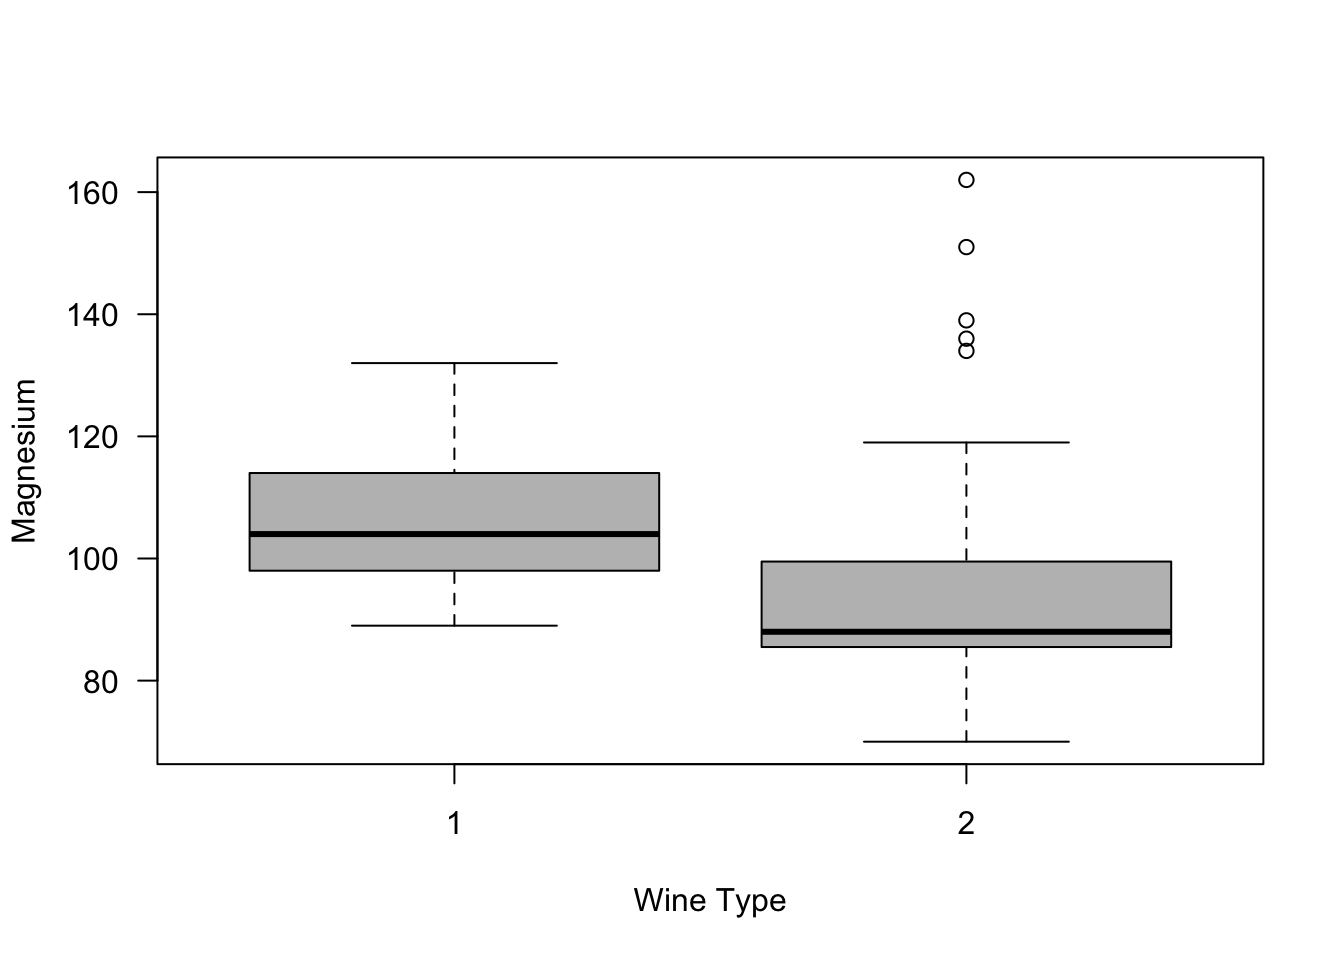
\includegraphics{03-rankstat_files/figure-latex/unnamed-chunk-6-2.pdf}
\item
  Suppose we are interested in testing whether or not magnesium levels in
  Type 1 wine are generally larger than magnesium levels in Type 2 wine.
  This can be done with the following code
\end{itemize}

\begin{Shaded}
\begin{Highlighting}[]
\KeywordTok{wilcox.test}\NormalTok{(}\DataTypeTok{x=}\NormalTok{wine2}\OperatorTok{$}\NormalTok{Magnesium[wine2}\OperatorTok{$}\NormalTok{Type}\OperatorTok{==}\DecValTok{1}\NormalTok{], }\DataTypeTok{y=}\NormalTok{wine2}\OperatorTok{$}\NormalTok{Magnesium[wine2}\OperatorTok{$}\NormalTok{Type}\OperatorTok{==}\DecValTok{2}\NormalTok{], }
            \DataTypeTok{alternative=}\StringTok{"greater"}\NormalTok{)}
\end{Highlighting}
\end{Shaded}

\begin{verbatim}
## 
##  Wilcoxon rank sum test with continuity correction
## 
## data:  wine2$Magnesium[wine2$Type == 1] and wine2$Magnesium[wine2$Type == 2]
## W = 3381.5, p-value = 8.71e-10
## alternative hypothesis: true location shift is greater than 0
\end{verbatim}

You could also use the following code (just be careful about the ordering of the levels of \textbf{Type})

\begin{Shaded}
\begin{Highlighting}[]
\KeywordTok{wilcox.test}\NormalTok{(Magnesium }\OperatorTok{~}\StringTok{ }\NormalTok{Type, }\DataTypeTok{data=}\NormalTok{wine2, }\DataTypeTok{alternative=}\StringTok{"greater"}\NormalTok{)}
\end{Highlighting}
\end{Shaded}

\begin{verbatim}
## 
##  Wilcoxon rank sum test with continuity correction
## 
## data:  Magnesium by Type
## W = 3381.5, p-value = 8.71e-10
## alternative hypothesis: true location shift is greater than 0
\end{verbatim}

\begin{itemize}
\tightlist
\item
  What is the value of the WRS test statistic? We can code this directly
  with the following steps:
\end{itemize}

\begin{Shaded}
\begin{Highlighting}[]
\NormalTok{W <-}\StringTok{ }\KeywordTok{wilcox.test}\NormalTok{(}\DataTypeTok{x=}\NormalTok{wine2}\OperatorTok{$}\NormalTok{Magnesium[wine2}\OperatorTok{$}\NormalTok{Type}\OperatorTok{==}\DecValTok{1}\NormalTok{], }\DataTypeTok{y=}\NormalTok{wine2}\OperatorTok{$}\NormalTok{Magnesium[wine2}\OperatorTok{$}\NormalTok{Type}\OperatorTok{==}\DecValTok{2}\NormalTok{])}

\NormalTok{n <-}\StringTok{ }\KeywordTok{sum}\NormalTok{(wine2}\OperatorTok{$}\NormalTok{Type}\OperatorTok{==}\DecValTok{1}\NormalTok{)}
\NormalTok{m <-}\StringTok{ }\KeywordTok{sum}\NormalTok{(wine2}\OperatorTok{$}\NormalTok{Type}\OperatorTok{==}\DecValTok{2}\NormalTok{)}
\NormalTok{zz <-}\StringTok{ }\KeywordTok{rank}\NormalTok{(wine2}\OperatorTok{$}\NormalTok{Magnesium) }\CommentTok{## vector of pooled ranks}
\KeywordTok{sum}\NormalTok{(zz[wine2}\OperatorTok{$}\NormalTok{Type}\OperatorTok{==}\DecValTok{1}\NormalTok{])  }\CommentTok{## The WRS test statistic}
\end{Highlighting}
\end{Shaded}

\begin{verbatim}
## [1] 5151.5
\end{verbatim}

\begin{itemize}
\tightlist
\item
  The statistic returned by the \textbf{wilcox.test} function is actually equal to \(W - n(n+1)/2\) not \(W\)
\end{itemize}

\begin{Shaded}
\begin{Highlighting}[]
\KeywordTok{sum}\NormalTok{(zz[wine2}\OperatorTok{$}\NormalTok{Type}\OperatorTok{==}\DecValTok{1}\NormalTok{]) }\OperatorTok{-}\StringTok{ }\NormalTok{n}\OperatorTok{*}\NormalTok{(n }\OperatorTok{+}\StringTok{ }\DecValTok{1}\NormalTok{)}\OperatorTok{/}\DecValTok{2}
\end{Highlighting}
\end{Shaded}

\begin{verbatim}
## [1] 3381.5
\end{verbatim}

\begin{Shaded}
\begin{Highlighting}[]
\NormalTok{W}\OperatorTok{$}\NormalTok{statistic}
\end{Highlighting}
\end{Shaded}

\begin{verbatim}
##      W 
## 3381.5
\end{verbatim}

\begin{itemize}
\tightlist
\item
  \(\{ W - n(n+1)/2 \}\) is equal to the Mann-Whitney statistic. Thus, \textbf{W\$statistic/(mn)} is
  an estimate of the probability \(P(X_{i} > Y_{j}) + P(X_{i} = Y_{j})/2\).
\end{itemize}

\begin{Shaded}
\begin{Highlighting}[]
\NormalTok{W}\OperatorTok{$}\NormalTok{statistic}\OperatorTok{/}\NormalTok{(m}\OperatorTok{*}\NormalTok{n)}
\end{Highlighting}
\end{Shaded}

\begin{verbatim}
##         W 
## 0.8072332
\end{verbatim}

\begin{itemize}
\tightlist
\item
  Let's check how the Mann-Whitney statistic matches a simulation-based estimate of this probability
\end{itemize}

\begin{Shaded}
\begin{Highlighting}[]
\NormalTok{ind1 <-}\StringTok{ }\KeywordTok{which}\NormalTok{(wine2}\OperatorTok{$}\NormalTok{Type}\OperatorTok{==}\DecValTok{1}\NormalTok{)}
\NormalTok{ind2 <-}\StringTok{ }\KeywordTok{which}\NormalTok{(wine2}\OperatorTok{$}\NormalTok{Type}\OperatorTok{==}\DecValTok{2}\NormalTok{)}
\NormalTok{xgreater <-}\StringTok{ }\KeywordTok{rep}\NormalTok{(}\DecValTok{0}\NormalTok{, }\DecValTok{100}\NormalTok{)}
\ControlFlowTok{for}\NormalTok{(k }\ControlFlowTok{in} \DecValTok{1}\OperatorTok{:}\DecValTok{100}\NormalTok{) \{}
\NormalTok{    xi <-}\StringTok{ }\KeywordTok{sample}\NormalTok{(ind1, }\DataTypeTok{size=}\DecValTok{1}\NormalTok{)}
\NormalTok{    yi <-}\StringTok{ }\KeywordTok{sample}\NormalTok{(ind2, }\DataTypeTok{size=}\DecValTok{1}\NormalTok{)}
\NormalTok{    xgreater[k] <-}\StringTok{ }\KeywordTok{ifelse}\NormalTok{(wine2}\OperatorTok{$}\NormalTok{Magnesium[xi] }\OperatorTok{>}\StringTok{ }\NormalTok{wine2}\OperatorTok{$}\NormalTok{Magnesium[yi], }\DecValTok{1}\NormalTok{, }\DecValTok{0}\NormalTok{) }\OperatorTok{+}\StringTok{ }
\StringTok{                   }\KeywordTok{ifelse}\NormalTok{(wine2}\OperatorTok{$}\NormalTok{Magnesium[xi] }\OperatorTok{==}\StringTok{ }\NormalTok{wine2}\OperatorTok{$}\NormalTok{Magnesium[yi], }\DecValTok{1}\OperatorTok{/}\DecValTok{2}\NormalTok{, }\DecValTok{0}\NormalTok{)}
\NormalTok{\}}
\KeywordTok{mean}\NormalTok{(xgreater)  }\CommentTok{## estimate of this probability}
\end{Highlighting}
\end{Shaded}

\begin{verbatim}
## [1] 0.79
\end{verbatim}

\hypertarget{additional-notes-for-the-wrs-test}{%
\subsection{Additional Notes for the WRS test}\label{additional-notes-for-the-wrs-test}}

\hypertarget{comparing-ordinal-data}{%
\subsubsection{Comparing Ordinal Data}\label{comparing-ordinal-data}}

\begin{itemize}
\item
  The WRS test is often suggested when comparing categorical data which are \textbf{ordinal}.
\item
  For example, we might have 4 categories:

  \begin{itemize}
  \tightlist
  \item
    Poor
  \item
    Fair
  \item
    Good
  \item
    Excellent
  \end{itemize}
\item
  In this case, there is a natural ordering of the categories
  but any numerical values assigned to these categories would be arbitrary.
\item
  In such cases, we might be interested in testing whether or not outcomes tend to be
  better in one group than the other rather than simply comparing whether or not
  the distribution is different between the two groups.
\item
  A WRS test is useful here since we can still compute ranks without having to
  choose aribtrary numbers for each category.
\item
  Thinking of the ``probability greater than alternative \eqref{eq:mw-formulation}''
  or ``stochastically larger than alternative \eqref{eq:stochasticlarger-formulation}'' interpretation
  of the WRS test is probably more reasonable than the ``shift alternative \eqref{eq:shift-formulation}'' interpretation.
\item
  Note that there will probably be many ties when comparing ordinal data.
\end{itemize}

\begin{center}\rule{0.5\linewidth}{\linethickness}\end{center}

\begin{itemize}
\item
  The Hodges-Lehmann Estimator \(\hat{\Delta}\) is an estimator of \(\Delta\) in the location-shift model
  \begin{equation}
  F_{X}(t) = F_{Y}(t - \Delta) \nonumber
  \end{equation}
\item
  The Hodges-Lehmann is defined as the median difference among all possible (group 1, group 2) pairs.
  Specifically,
  \begin{equation}
  \hat{\Delta} = \textrm{median}\{ (X_{i} - Y_{j}); i=1,\ldots,n; j=1,\ldots,m \} \nonumber
  \end{equation}
\item
  We won't discuss the Hodges-Lehmann estimator in detail in this course, but in
  many statistical software packages, the
  Hodges-Lehmann is often reported when computing the WRS test.
\item
  In \textbf{R}, the Hodges-Lehmann estimator can be obtained by using the \textbf{conf.int=TRUE}
  argument in the \textbf{wilcox.test} function
\end{itemize}

\begin{Shaded}
\begin{Highlighting}[]
\NormalTok{WC <-}\StringTok{ }\KeywordTok{wilcox.test}\NormalTok{(}\DataTypeTok{x=}\NormalTok{wine2}\OperatorTok{$}\NormalTok{Magnesium[wine2}\OperatorTok{$}\NormalTok{Type}\OperatorTok{==}\DecValTok{1}\NormalTok{], }\DataTypeTok{y=}\NormalTok{wine2}\OperatorTok{$}\NormalTok{Magnesium[wine2}\OperatorTok{$}\NormalTok{Type}\OperatorTok{==}\DecValTok{2}\NormalTok{],}
                  \DataTypeTok{conf.int=}\OtherTok{TRUE}\NormalTok{)}
\NormalTok{WC}\OperatorTok{$}\NormalTok{estimate     }\CommentTok{## The Hodges-Lehmann estimate}
\end{Highlighting}
\end{Shaded}

\begin{verbatim}
## difference in location 
##               14.00005
\end{verbatim}

\hypertarget{one-sample-tests}{%
\section{One Sample Tests}\label{one-sample-tests}}

\hypertarget{sign-test}{%
\subsection{The Sign Test}\label{sign-test}}

\hypertarget{motivation-and-definition}{%
\subsubsection{Motivation and Definition}\label{motivation-and-definition}}

\begin{itemize}
\item
  The \textbf{sign test} can be thought of as a test of whether or not
  the median of a distribution is greater than zero (or greater than some other fixed value \(\theta_{0}\)).
\item
  Frequently, the sign test is explained in the following context:

  \begin{itemize}
  \tightlist
  \item
    Suppose we have observations \(D_{1}, \ldots, D_{n}\) which arise from the model
    \begin{equation}
    D_{i} = \theta + \varepsilon_{i},
    \label{eq:general-location}
    \end{equation}
    where \(\varepsilon_{i}\) are iid random variables each with distribution function \(F_{\epsilon}\)
    that is assumed to have a median of zero. Moreover, we will assume the density function
    \(f_{\varepsilon}(t)\) is symmetric around zero.
  \end{itemize}
\item
  The distribution function of \(D_{i}\) is then
  \begin{equation}
  F_{D}(t) = P(D_{i} \leq t) = P(\varepsilon_{i} \leq t - \theta) = F_{\epsilon}(t - \theta)
  \end{equation}
\item
  Likewise the density function \(f_{D}(t)\) of \(D_{i}\) is given by
  \begin{equation}
  f_{D}(t) = f_{\epsilon}(t - \theta)
  \end{equation}
\item
  In this context, \(\theta\) is usually referred to as a \textbf{location parameter}.
\item
  The goal here is to test \(H_{0}: \theta = \theta_{0}\) vs. \(H_{A}: \theta > \theta_{0}\). (Often, \(\theta_{0} = 0\)).
\end{itemize}

\begin{center}\rule{0.5\linewidth}{\linethickness}\end{center}

\begin{itemize}
\tightlist
\item
  This sort of test usually comes up in the context of \textbf{paired data}.
  Common examples include

  \begin{itemize}
  \tightlist
  \item
    patients compared ``pre and post treatment''
  \item
    students before and after the introduction of a new teaching method
  \item
    comparison of ``matched'' individuals who are similar (e.g., same age, sex, education, etc.)
  \item
    comparing consistency of measurements made on the same objects
  \end{itemize}
\end{itemize}

Baseline\_Measure

Post\_Treatment\_Measure

Patient 1

Y1

X1

Patient 2

Y2

X2

Patient 3

Y3

X3

Patient 4

Y4

X4

\begin{itemize}
\item
  In such cases, we have observations \(X_{i}\) and \(Y_{i}\) for \(i = 1,\ldots n\) where
  it is not necessarily reasonable to think of \(X_{i}\) and \(Y_{i}\) as independent.
\item
  We can define \(D_{i} = X_{i} - Y_{i}\) as the difference in the \(i^{th}\) pair.
\item
  With this setup, a natural question is whether or not the differences \(D_{i}\) tend to be
  greater than zero or not.
\end{itemize}

\begin{center}\rule{0.5\linewidth}{\linethickness}\end{center}

\begin{itemize}
\item
  The \textbf{sign} statistic \(S_{n}\) is defined as
  \begin{equation}
  S_{n} = \sum_{i=1}^{n} I( D_{i} > 0)
  \label{eq:sign-statistic}
  \end{equation}
\item
  If the null hypothesis \(H_{0}: \theta = 0\) is true, then we should expect that roughly half
  of the observations will be positive.
\item
  This suggests that we will reject \(H_{0}\) if \(S_{n} \geq c\) where \(c\) is a
  number that is greater than \(n/2\).
\end{itemize}

\hypertarget{null-distribution-and-p-values}{%
\subsubsection{Null Distribution and p-values}\label{null-distribution-and-p-values}}

\begin{itemize}
\item
  Notice that the sign statistic defined in \eqref{eq:sign-statistic} is the sum of independent
  Bernoulli random variable.
\item
  That is, we can think of \(Z_{i} = I(D_{i} > 0)\) as a random variable with success probability
  \(p( \theta )\) where the formula for \(p( \theta )\) is
  \begin{equation}
  p(\theta) = P(Z_{i} = 1) = P(D_{i} > 0) = 1 - F_{D}(0) = 1 - F_{\epsilon}( -\theta )
  \end{equation}
\item
  This implies that \(S_{n}\) is a binomial random variable
  with \(n\) trials and success probability \(p(\theta)\).
  That is,
  \begin{equation}
  S_{n} \sim \textrm{Binomial}(n, p(\theta) )
  \label{eq:signstat-distribution}
  \end{equation}
\item
  Because \(p(0) = 1/2\), \(S_{n} \sim \textrm{Binomial}(n, 1/2 )\) under \(H_{0}\).
\item
  Notice that the ``null distribution'' of the sign statistic is ``distribution free''
  in the sense that the distribution does not depend on the distribution of \(D_{i}\).
\item
  The p-value for the sign test can be computed by
  \begin{equation}
  \textrm{p-value} = P_{H_{0}}(S_{n} \geq s_{obs}) = \sum_{j=s_{obs}}^{n} P_{H_{0}}(S_{n} = j)
  = \sum_{j=s_{obs}}^{n} {n \choose j} \frac{1}{2^{n}},
  \end{equation}
  where \(s_{obs}\) is the observed value of the sign statistic.
\end{itemize}

\begin{Shaded}
\begin{Highlighting}[]
\CommentTok{### How to compute the p-value for the sign test using R}
\NormalTok{xx <-}\StringTok{ }\KeywordTok{rnorm}\NormalTok{(}\DecValTok{100}\NormalTok{)}
\NormalTok{sign.stat <-}\StringTok{ }\KeywordTok{sum}\NormalTok{(xx }\OperatorTok{>}\StringTok{ }\DecValTok{0}\NormalTok{)}
\DecValTok{1} \OperatorTok{-}\StringTok{ }\KeywordTok{pbinom}\NormalTok{(sign.stat }\OperatorTok{-}\StringTok{ }\DecValTok{1}\NormalTok{, }\DataTypeTok{size=}\DecValTok{100}\NormalTok{, }\DataTypeTok{prob=}\DecValTok{1}\OperatorTok{/}\DecValTok{2}\NormalTok{) }\CommentTok{## p-value for sign test}
\end{Highlighting}
\end{Shaded}

\begin{verbatim}
## [1] 0.6178233
\end{verbatim}

\begin{itemize}
\item
  The reason that this is the right expression using \textbf{R} is that for any positive integer \(w\)
  \begin{equation}
  P_{H_{0}}(S_{n} \geq w) = 1 - P_{H_{0}}(S_{n} < w) = 1 - P_{H_{0}}(S_{n} \leq w - 1)
  \end{equation}
  and the \textbf{R} function \textbf{pbinom(t, n, prob)} computes \(P(X \leq t)\) where \(X\) is
  a binomial random variable with \(n\) trials and success probability \textbf{prob}.
\item
  You can also perform the one-sided sign test by using the \textbf{binom.test} function in \textbf{R}.
\end{itemize}

\begin{Shaded}
\begin{Highlighting}[]
\NormalTok{btest <-}\StringTok{ }\KeywordTok{binom.test}\NormalTok{(sign.stat, }\DataTypeTok{n=}\DecValTok{100}\NormalTok{, }\DataTypeTok{p=}\FloatTok{0.5}\NormalTok{, }\DataTypeTok{alternative=}\StringTok{"greater"}\NormalTok{) }
\NormalTok{btest}\OperatorTok{$}\NormalTok{p.value}
\end{Highlighting}
\end{Shaded}

\begin{verbatim}
## [1] 0.6178233
\end{verbatim}

\hypertarget{two-sided-sign-test}{%
\subsubsection{Two-sided Sign Test}\label{two-sided-sign-test}}

\begin{itemize}
\item
  Notice that the number of negative values of \(D_{i}\) can be expressed as
  \begin{equation}
  \sum_{i=1}^{n} I(D_{i} < 0) = n - S_{n}
  \end{equation}
  if there are no observations that equal zero exactly. Large value of \(n - S_{n}\)
  would be used in favor of another possible one-sided alternative \(H_{A}: \theta < 0\).
\item
  If we now want to test the two-sided alternative
  \begin{equation}
  H_{0}: \theta = 0 \quad \textrm{ vs. }  \quad H_{A}: \theta \neq 0 \nonumber
  \end{equation}
  you would need to compute the probability under the null hypothesis of observing
  a ``more extreme'' observation than the one that was actually observed.
\item
  Extreme is defined by thinking about the fact that we would have rejected \(H_{0}\)
  if either \(S_{n}\) or \(n - S_{n}\) were very large.
\item
  For example, if \(n = 12\), then the expected value of the sign statistic would be \(6\).
  If \(s_{obs} = 10\), then the collection of ``more extreme'' events then this would be
  \(\leq 2\) and \(\geq 10\).
\item
  The two-sided p-value is determined by looking at the tail probabilities on both sides
  \begin{equation}
  \textrm{p-value} = 
  \begin{cases}
  P_{H_{0}}(S_{n} \geq s_{obs}) + P_{H_{0}}(S_{n} \leq n - s_{obs}) & \textrm{ if } s_{obs} \geq n/2 \\
  P_{H_{0}}(S_{n} \leq s_{obs}) + P_{H_{0}}(S_{n} \geq n - s_{obs}) & \textrm{ if } s_{obs} < n/2
  \end{cases}
  \end{equation}
\item
  It actually works out that
  \begin{equation}
  \textrm{p-value} = 
  \begin{cases}
  2 P_{H_{0}}(S_{n} \geq s_{obs})   & \textrm{ if } s_{obs} \geq n/2 \\
  2 P_{H_{0}}(S_{n} \leq s_{obs})   & \textrm{ if } s_{obs} < n/2
  \end{cases}
  \end{equation}
\item
  Also, you can note that this p-value would be the same that you would get from performing the test
  \(H_{0}: p = 1/2\) vs. \(H_{A}: p \neq 1/2\) when it is assumed that \(S_{n} \sim \textrm{Binomial}(n, p)\).
\item
  Another note: It is often suggested that one should drop observations which are exactly zero
  when performing the sign test.
\end{itemize}

\hypertarget{the-wilcoxon-signed-rank-test}{%
\subsection{The Wilcoxon Signed Rank Test}\label{the-wilcoxon-signed-rank-test}}

\begin{itemize}
\item
  The Wilcoxon signed rank test can be applied
  under the same scenario that we used the sign test.
\item
  One criticism of the sign test is that it ignores the magnitude
  of the observations.
\item
  For example, the sign test statistic \(S\) treats observations
  \(D_{i} = 0.2\) and \(D_{i}=3\) the same.
\item
  The \textbf{Wilcoxon signed rank statistic} \(T_{n}\) weights the
  signs of \(D_{i}\) by the rank of its absolute value.
\item
  Specifically, the Wilcoxon signed rank statistic is defined as
  \begin{equation}
  T_{n} = \sum_{i=1}^{n} \textrm{sign}( D_{i}) R_{i}( |\mathbf{D}| )
  \end{equation}
  where the \(\textrm{sign}\) function is defined as
  \begin{equation}
  \textrm{sign}(x) = \begin{cases}
  1 & \textrm{if } x > 0 \\
  0 & \textrm{if } x = 0 \\
  -1 & \textrm{if } x < 0
  \end{cases}
  \end{equation}
\item
  Here, \(R_{i}( |\mathbf{D}| )\) is the rank of the \(i^{th}\) element from the vector
  \(|\mathbf{D}| = (|D_{1}|, |D_{2}|, \ldots, |D_{n}|)\).
\item
  Intuitively, the Wilcoxon signed rank statistic is measuring whether
  or not large values of \(|D_{i}|\) tend to be associated with positive
  vs.~negative values of \(D_{i}\).
\end{itemize}

\begin{center}\rule{0.5\linewidth}{\linethickness}\end{center}

Discuss some of these in class

\textbf{Exercise 3.4.} Suppose we had data \((-2, 1, -1/2, 3/2, 3)\). What would
be the value of the Wilcoxon signed rank statistic?

\textbf{Exercise 3.5.} Under the assumptions of model \eqref{eq:general-location}, what is
the density function of \(|D_{i}|\) and \(-|D_{i}|\)?

\textbf{Exercise 3.6.} Under the assumptions of model \eqref{eq:general-location} and
assuming that \(\theta = 0\), show that the expectation of the Wilcoxon signed-rank
statistic is \(0\).

\begin{center}\rule{0.5\linewidth}{\linethickness}\end{center}

\hypertarget{asymptotic-distribution}{%
\subsubsection{Asymptotic Distribution}\label{asymptotic-distribution}}

\begin{itemize}
\item
  As mentioned in the above exercise, the expectation of \(T_{n}\) under \(H_{0}\) is zero.
\item
  It can be shown that the variance under the null hypothesis is
  \begin{equation}
  \textrm{Var}_{H_{0}}( T_{n} ) = \frac{n(2n + 1)(n + 1)}{6} \nonumber
  \end{equation}
\item
  Similar, to the large-sample approximation we used for the WRS test, we have the following
  asymptotic result for the Wilcoxon signed-rank test
  \begin{equation}
  \frac{T_{n}}{\sqrt{\textrm{Var}_{H_{0}}(T_{n}) }} \longrightarrow \textrm{Normal}(0,1) \quad \textrm{as } n \longrightarrow \infty
  \end{equation}
\item
  Because the variance of \(T\) is dominated by the term \(n^{3}/3\) for very large \(n\), we could also say that under \(H_{0}\)
  that
  \begin{equation}
  \frac{T_{n}}{\sqrt{n^{3}/3} } \longrightarrow \textrm{Normal}(0,1) \quad \textrm{as } n \longrightarrow \infty
  \end{equation}
  In other words, we can say that \(T_{n}\) has an approximately \(\textrm{Normal}(0, n^{3}/3)\) for large \(n\).
\end{itemize}

\hypertarget{exact-distribution}{%
\subsubsection{Exact Distribution}\label{exact-distribution}}

\begin{itemize}
\tightlist
\item
  The exact distribution of the Wilcoxon signed rank statistic \(T_{n}\)
  is somewhat more complicated than the exact distribution of the WRS test statistic.
  Nevertheless, there exists functions in \textbf{R} for working with this exact distribution.
\end{itemize}

\hypertarget{using-r-to-perform-the-sign-and-wilcoxon-tests}{%
\subsection{Using R to Perform the Sign and Wilcoxon Tests}\label{using-r-to-perform-the-sign-and-wilcoxon-tests}}

\begin{itemize}
\item
  Let's first look at the \textbf{Meat} data from the \textbf{PairedData} \textbf{R} package.
\item
  This data set contains 20 observations with measures of fat percentage using different
  measuring techniques.
\end{itemize}

\begin{Shaded}
\begin{Highlighting}[]
\KeywordTok{library}\NormalTok{(PairedData, }\DataTypeTok{quietly=}\OtherTok{TRUE}\NormalTok{, }\DataTypeTok{warn.conflicts=}\OtherTok{FALSE}\NormalTok{) }\CommentTok{## loading PairedData package}
\KeywordTok{data}\NormalTok{(Meat)  }\CommentTok{## loading Meat data}
\KeywordTok{head}\NormalTok{(Meat)}
\end{Highlighting}
\end{Shaded}

\begin{verbatim}
##   AOAC Babcock     MeatType
## 1 22.0    22.3       Wiener
## 2 22.1    21.8       Wiener
## 3 22.1    22.4       Wiener
## 4 22.2    22.5       Wiener
## 5 24.6    24.9   ChoppedHam
## 6 25.3    25.6 ChooppedPork
\end{verbatim}

\begin{itemize}
\tightlist
\item
  Define the differences \(D_{i}\) as the \textbf{Babcock} measurements minus the \textbf{AOAC} measures.
  We will drop the single observation that equals zero.
\end{itemize}

\begin{Shaded}
\begin{Highlighting}[]
\NormalTok{DD <-}\StringTok{ }\NormalTok{Meat[,}\DecValTok{2}\NormalTok{] }\OperatorTok{-}\StringTok{ }\NormalTok{Meat[,}\DecValTok{1}\NormalTok{]}
\NormalTok{DD <-}\StringTok{ }\NormalTok{DD[DD}\OperatorTok{!=}\DecValTok{0}\NormalTok{]}
\KeywordTok{hist}\NormalTok{(DD, }\DataTypeTok{main=}\StringTok{"Meat Data"}\NormalTok{, }\DataTypeTok{xlab=}\StringTok{"Difference in Measured Fat Percentage"}\NormalTok{, }\DataTypeTok{las=}\DecValTok{1}\NormalTok{)}
\end{Highlighting}
\end{Shaded}

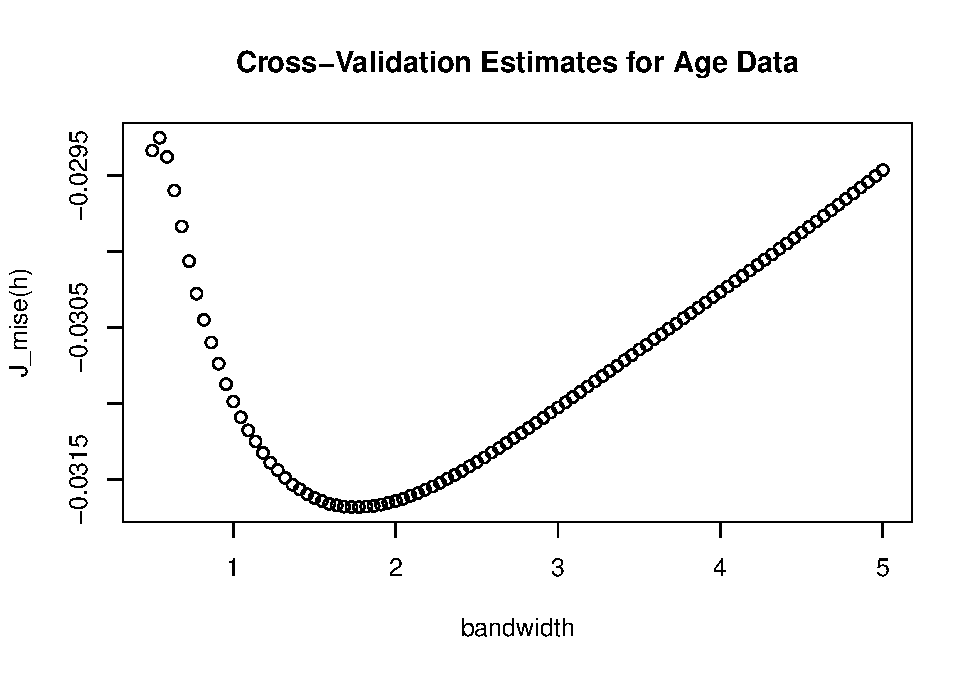
\includegraphics{03-rankstat_files/figure-latex/unnamed-chunk-17-1.pdf}

\begin{Shaded}
\begin{Highlighting}[]
\KeywordTok{summary}\NormalTok{(DD)}
\end{Highlighting}
\end{Shaded}

\begin{verbatim}
##     Min.  1st Qu.   Median     Mean  3rd Qu.     Max. 
## -1.60000 -0.25000  0.30000  0.04211  0.40000  1.10000
\end{verbatim}

\textbf{The Sign Test in R}

\begin{itemize}
\tightlist
\item
  Let's first test the hypothesis \(H_{0}: \theta = 0\) vs. \(H_{A}: \theta \neq 0\) using
  the two-sided sign test. This can be done using the \textbf{binom.test} function
\end{itemize}

\begin{Shaded}
\begin{Highlighting}[]
\KeywordTok{binom.test}\NormalTok{(}\KeywordTok{sum}\NormalTok{(DD }\OperatorTok{>}\StringTok{ }\DecValTok{0}\NormalTok{), }\DataTypeTok{n =} \KeywordTok{length}\NormalTok{(DD), }\DataTypeTok{p=}\FloatTok{0.5}\NormalTok{)}\OperatorTok{$}\NormalTok{p.value}
\end{Highlighting}
\end{Shaded}

\begin{verbatim}
## [1] 0.6476059
\end{verbatim}

\textbf{Wilcoxon Signed Rank Test in R}

\begin{itemize}
\tightlist
\item
  You can actually use the function \textbf{wilcox.test} to perform the Wilcoxon signed rank test in addition
  to the Wilcoxon rank sum test. To perform the Wilcoxon signed rank test in \textbf{R}, you just
  need to enter data for the \textbf{x} argument and leave the \textbf{y} argument empty.
\end{itemize}

\begin{Shaded}
\begin{Highlighting}[]
\KeywordTok{wilcox.test}\NormalTok{(}\DataTypeTok{x=}\NormalTok{DD)}
\end{Highlighting}
\end{Shaded}

\begin{verbatim}
## Warning in wilcox.test.default(x = DD): cannot compute exact p-value with ties
\end{verbatim}

\begin{verbatim}
## 
##  Wilcoxon signed rank test with continuity correction
## 
## data:  DD
## V = 118.5, p-value = 0.3534
## alternative hypothesis: true location is not equal to 0
\end{verbatim}

\begin{itemize}
\item
  You will note that the p-value for the Wilcoxon signed rank test is lower than that
  of the sign test. In general, the Wilcoxon signed rank test is somewhat more ``sensitive''
  than the sign test meaning that it will have a greater tendency
  to reject \(H_{0}\) for small deviations from \(H_{0}\).
\item
  We can explore this sensitivity comparison with a small simulation study. We
  will consider a scenario where \(D_{i} = 0.4 + \varepsilon_{i}\) with \(\varepsilon_{i}\)
  having a t distribution with \(3\) degrees of freedom.
\end{itemize}

\begin{Shaded}
\begin{Highlighting}[]
\KeywordTok{set.seed}\NormalTok{(}\DecValTok{1327}\NormalTok{)}
\NormalTok{n.reps <-}\StringTok{ }\DecValTok{500}  \CommentTok{## number of simulation replications}
\NormalTok{samp.size <-}\StringTok{ }\DecValTok{50}  \CommentTok{## the sample size}
\NormalTok{wilcox.reject <-}\StringTok{ }\KeywordTok{rep}\NormalTok{(}\DecValTok{0}\NormalTok{, n.reps)}
\NormalTok{sign.reject <-}\StringTok{ }\KeywordTok{rep}\NormalTok{(}\DecValTok{0}\NormalTok{, n.reps)}
\ControlFlowTok{for}\NormalTok{(k }\ControlFlowTok{in} \DecValTok{1}\OperatorTok{:}\NormalTok{n.reps) \{}
\NormalTok{    dsim <-}\StringTok{ }\FloatTok{.4} \OperatorTok{+}\StringTok{ }\KeywordTok{rt}\NormalTok{(samp.size, }\DataTypeTok{df=}\DecValTok{3}\NormalTok{)}
\NormalTok{    wilcox.reject[k] <-}\StringTok{ }\KeywordTok{ifelse}\NormalTok{(}\KeywordTok{wilcox.test}\NormalTok{(}\DataTypeTok{x=}\NormalTok{dsim)}\OperatorTok{$}\NormalTok{p.value }\OperatorTok{<}\StringTok{ }\FloatTok{0.05}\NormalTok{, }\DecValTok{1}\NormalTok{, }\DecValTok{0}\NormalTok{)}
\NormalTok{    sign.reject[k] <-}\StringTok{ }\KeywordTok{ifelse}\NormalTok{(}\KeywordTok{binom.test}\NormalTok{(}\KeywordTok{sum}\NormalTok{(dsim }\OperatorTok{>}\StringTok{ }\DecValTok{0}\NormalTok{), }
                                       \DataTypeTok{n=}\NormalTok{samp.size, }\DataTypeTok{p=}\FloatTok{0.5}\NormalTok{)}\OperatorTok{$}\NormalTok{p.value }\OperatorTok{<}\StringTok{ }\FloatTok{0.05}\NormalTok{, }\DecValTok{1}\NormalTok{, }\DecValTok{0}\NormalTok{)}
\NormalTok{\}}
\KeywordTok{mean}\NormalTok{(wilcox.reject)  }\CommentTok{## proportion of times Wilcoxon signed rank rejected H0}
\end{Highlighting}
\end{Shaded}

\begin{verbatim}
## [1] 0.614
\end{verbatim}

\begin{Shaded}
\begin{Highlighting}[]
\KeywordTok{mean}\NormalTok{(sign.reject)  }\CommentTok{## proportion of times Wilcoxon signed rank rejected H0}
\end{Highlighting}
\end{Shaded}

\begin{verbatim}
## [1] 0.488
\end{verbatim}

\hypertarget{power-and-comparisons-with-parametric-tests}{%
\section{Power and Comparisons with Parametric Tests}\label{power-and-comparisons-with-parametric-tests}}

\hypertarget{the-power-function-of-a-test}{%
\subsection{The Power Function of a Test}\label{the-power-function-of-a-test}}

\begin{itemize}
\item
  The \textbf{power} of a test is the probability
  that a test rejects the null hypothesis when the
  alternative hypothesis is true.
\item
  The alternative hypothesis \(H_{A}\) is usually characterized
  by a large range of values of the parameter of interest.
  For example, \(H_{A}: \theta > 0\) or \(H_{A}: \theta \neq 0\).
\item
  For this reason, it is better to think of power
  as a function that varies across the range
  of the alternative hypothesis.
\item
  To be more precise, we will define the power
  function as a function of some parameter \(\theta\)
  where the null hypothesis corresponds to \(\theta = \theta_{0}\)
  and the alternative hypothesis represents a range
  of alternative values of \(\theta\).
\item
  The power function \(\gamma_{n}(\cdot)\) of a testing procedure is defined as
  \begin{equation}
  \gamma_{n}(\delta) = P_{\theta=\delta}\{  \textrm{reject } H_{0} \} \qquad \textrm{ for } \delta \in H_{A}. \nonumber
  \end{equation}
\item
  The notation \(P_{\theta=\delta}\{ \textrm{reject } H_{0} \}\) means that we are computing this
  probability under the assumption that the parameter of interest \(\theta\) equals \(\delta\).
\end{itemize}

\begin{center}\rule{0.5\linewidth}{\linethickness}\end{center}

\textbf{The Approximate Power Function of the Sign Test}

\begin{itemize}
\item
  Let us consider the sign test for testing \(H_{0}: \theta = 0\) vs. \(\theta > 0\).
\item
  The sign test is based on the value of the sign statistic \(S_{n}\).
\item
  Recalling \eqref{eq:signstat-distribution}, we know that \(S_{n} \sim \textrm{Binomial}(n, p(\theta))\).
  Hence,
  \begin{equation}
  \sqrt{n}(\tfrac{S_{n}}{n} - p(\theta)) \longrightarrow \textrm{Normal}\Big( 0, p(\theta)(1 - p(\theta)) \Big) \quad \textrm{as } n \longrightarrow \infty
  \label{eq:approx-signstat}
  \end{equation}
\item
  The sign test will reject \(H_{0}\) when \(S_{n} \geq c_{\alpha,n}\) where the constant \(c_{\alpha,n}\) is chosen
  so that \(P_{H_{0}}( S_{n} \geq c_{\alpha,n} ) = \alpha\). Using the large-sample approximation \eqref{eq:approx-signstat}, you can
  show that
  \begin{equation}
  c_{\alpha, n} = \frac{n + \sqrt{n}z_{1-\alpha}}{2}, 
  \label{eq:critical-value-signstat}
  \end{equation}
  where \(z_{1-\alpha}\) denotes the upper \(1 - \alpha\) quantile of the standard normal distribution. In other words,
  \(\Phi( z_{1-\alpha}) = 1-\alpha\).
\item
  Also, when using large-sample approximation \eqref{eq:approx-signstat}, the power of this test to detect a value of \(\theta = \delta\) is given by
  \begin{eqnarray}
  \gamma_{n}(\delta) &=& P_{\theta=\delta}\{ S_{n} \geq c_{\alpha,n} \} 
  = P_{\theta=\delta}\Bigg\{ \frac{\sqrt{n}(S_{n}/n - p(\delta))}{\sqrt{ p(\delta)(1 - p(\delta)) } } \geq 
  \frac{ \sqrt{n}(c_{\alpha, n}/n - p(\delta)) }{ \sqrt{p(\delta)(1 - p(\delta))}  } \Bigg\}  \nonumber \\
  &=& 1 - \Phi\Bigg( \frac{ \sqrt{n}(c_{\alpha,n}/n - p(\delta)) }{ \sqrt{p(\delta)(1 - p(\delta))}  } \Bigg) \nonumber \\
  &=& 1 - \Phi\Bigg( \frac{ z_{1-\alpha} }{ 2\sqrt{p(\delta)(1 - p(\delta))}  } - \frac{ \sqrt{n}(p(\delta) - 1/2) }{ \sqrt{p(\delta)(1 - p(\delta))}  }\Bigg)
  \label{eq:powerfn-signstat}
  \end{eqnarray}
\item
  Notice that the power of the test depends more directly on the term \(p(\delta) = P_{\theta = \delta}(D_{i} > 0)\).
  Recall from Section \ref{sign-test} that
  \(p(\delta) = 1 - F_{\epsilon}(\delta)\), where \(F_{\epsilon}\) is the distribution function
  of \(\varepsilon_{i}\) in the model \(D_{i} = \theta + \varepsilon_{i}\).
\item
  So, in any power or sample size calculation, it would be more sensible to think about plausible
  values for \(p(\delta)\) rather than \(\delta\) itself. Plus, \(p(\delta)\) has the direct interpretation
  \(p(\delta) = P_{\theta=\delta}( D_{i} > 0)\).
\end{itemize}

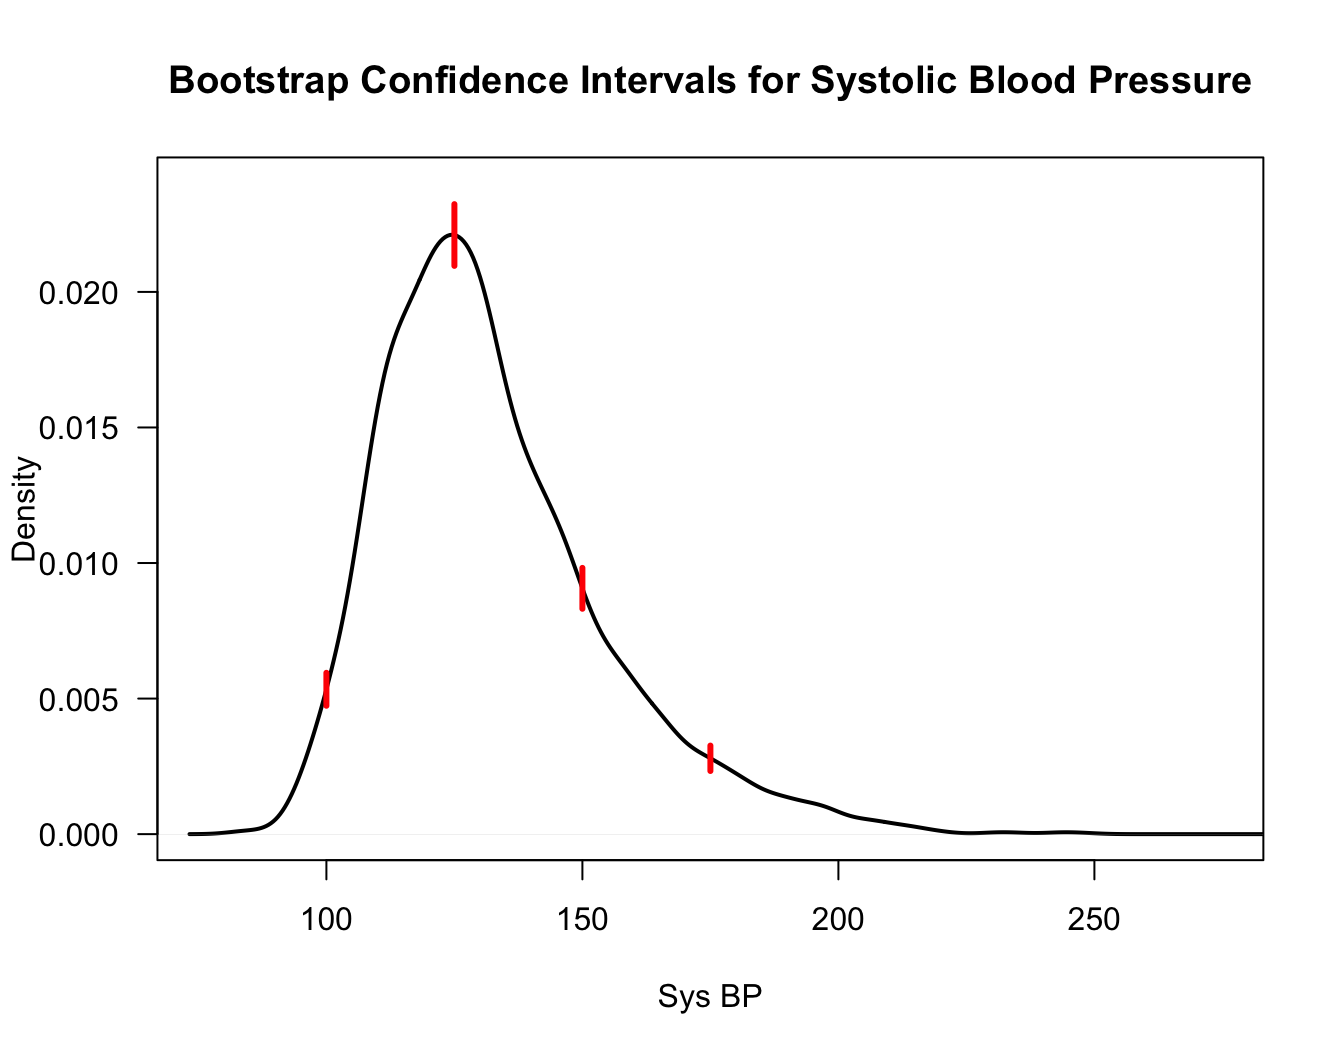
\includegraphics{03-rankstat_files/figure-latex/unnamed-chunk-21-1.pdf} 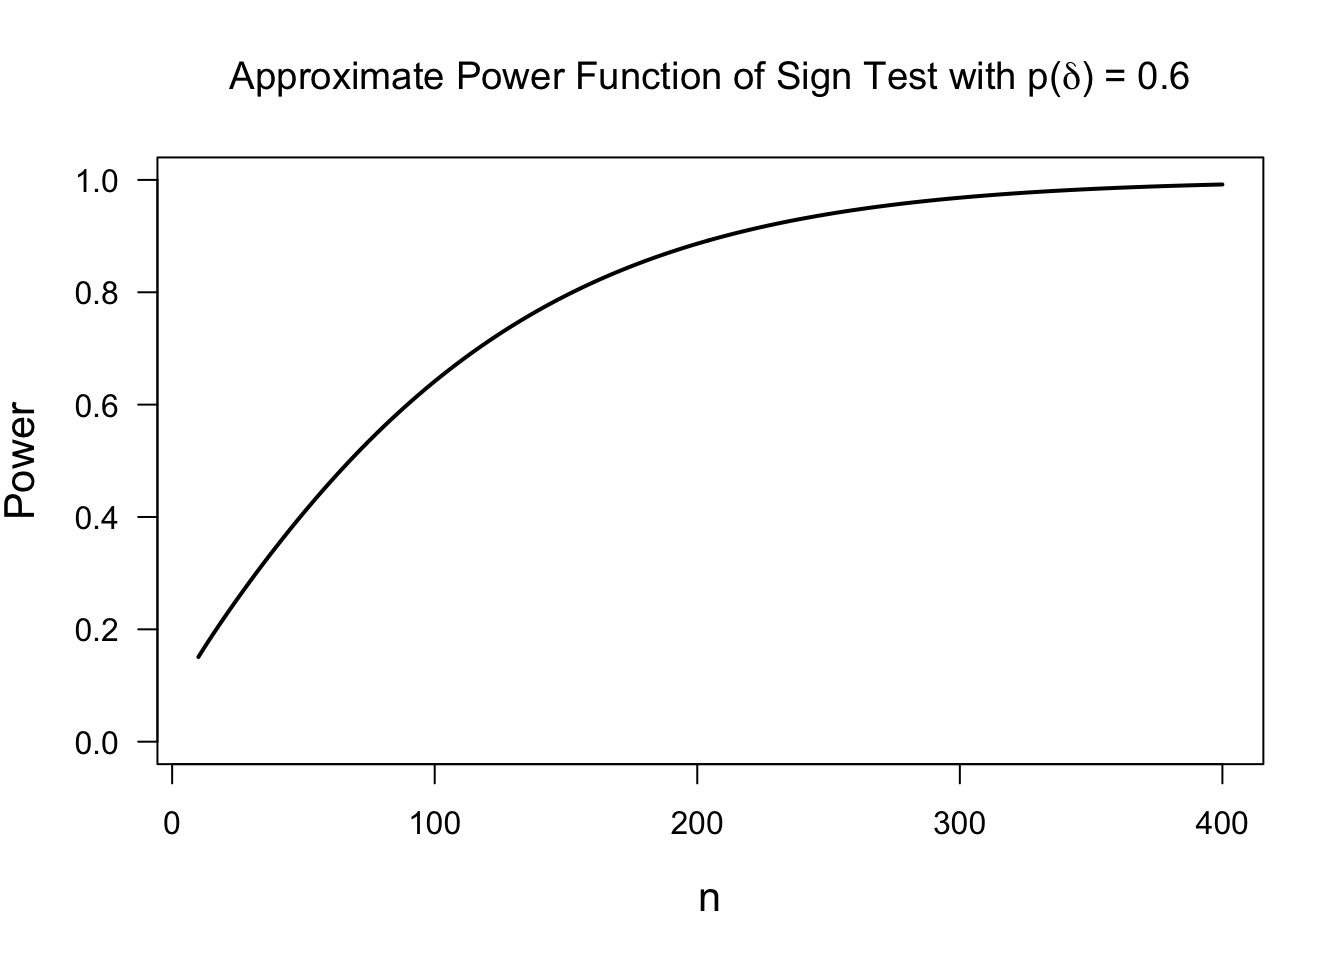
\includegraphics{03-rankstat_files/figure-latex/unnamed-chunk-21-2.pdf}

\begin{center}\rule{0.5\linewidth}{\linethickness}\end{center}

\textbf{Exercise 3.7}: Derive the formula for \(c_{\alpha, n}\) shown in \eqref{eq:critical-value-signstat}.

\begin{center}\rule{0.5\linewidth}{\linethickness}\end{center}

\hypertarget{power-comparisons-and-asymptotic-relative-efficiency}{%
\subsection{Power Comparisons and Asymptotic Relative Efficiency}\label{power-comparisons-and-asymptotic-relative-efficiency}}

\begin{itemize}
\item
  Notice that for the sign statistic power function shown in \eqref{eq:powerfn-signstat},
  we have that
  \begin{equation}
  \lim_{n \longrightarrow \infty} \gamma_{n}(\delta)
  = \begin{cases}
  \alpha & \textrm{ if } \delta = 0 \\
  1 & \textrm{ if } \delta > 0
  \end{cases}
  \label{eq:powerfn-consistent}
  \end{equation}
\item
  The above type of limit for the power function is will be
  true for most ``reasonable'' tests.
\item
  Indeed, a test whose power function satisfies
  \eqref{eq:powerfn-consistent} is typically called a \textbf{consistent} tests.
\end{itemize}

\begin{center}\rule{0.5\linewidth}{\linethickness}\end{center}

\begin{itemize}
\item
  If nearly all reasonable tests are consistent, then
  how can we compare tests with respect to their power?
\item
  One approach is to use simulations to compare power for several plausible alternatives.
  While this can be useful for a specific application, it limits
  our ability to make more general statements about power comparisons.
\item
  Another approach might be to determine
  for which values of \((\delta, n)\) one test has
  greater power than another. However, this could
  be tough to interpret (no test will be uniformly more powerful for all distributions)
  or even difficult to compute.
\item
  One way to think about power is to think about the \textbf{relative efficiency} of
  two testing procedures. The efficiency of a test in this context is
  the sample size required to achieve a certain level of power.
\end{itemize}

\begin{center}\rule{0.5\linewidth}{\linethickness}\end{center}

\begin{itemize}
\item
  To find the asymptotic relative efficiency, we first need to derive the
  asymptotic power function.
\item
  For our hypothesis \(H_{0}: \theta = \theta_{0}\) vs. \(H_{A}: \theta > \theta_{0}\), this is defined as
  \begin{equation}
  \tilde{\gamma}(\delta) = \lim_{n \longrightarrow \infty} \gamma_{n}( \theta_{0} + \delta/\sqrt{n}) \nonumber
  \end{equation}
\item
  Considering the sequence of ``local alternatives'' \(\theta_{n} = \theta_{0} + \delta/\sqrt{n}\),
  we avoid the problem of the power always converging to \(1\).
\item
  It can be shown that
  \begin{equation}
  \tilde{\gamma}(\delta) = 1 - \Phi\Bigg( z_{1-\alpha} - \delta \frac{\mu'(\theta_{0})}{\sigma(\theta_{0})} \Bigg)
  \end{equation}
  as long as we can find functions \(\mu(\cdot)\) and \(\sigma(\cdot)\) such that
  \begin{equation}
  \frac{\sqrt{n}(V_{n} - \mu(\theta_{n}))}{ \sigma(\theta_{n})} \longrightarrow \textrm{Normal}(0, 1) 
  \label{eq:asymptotic-v}
  \end{equation}
  where the test of \(H_{0}:\theta = \theta_{0}\) vs. \(H_{A}: \theta > \theta_{0}\)
  is based on the test statistic \(V_{n}\) with rejection of \(H_{0}\) occurring whenever \(V_{n} \geq c_{\alpha, n}\).
  Statement \eqref{eq:asymptotic-v} asssumes that the distribution of \(V_{n}\) is governed by \(\theta_{n}\) for each \(n\).
\end{itemize}

\begin{center}\rule{0.5\linewidth}{\linethickness}\end{center}

\begin{itemize}
\item
  The ratio \(e(\theta_{0}) = \mu'(\theta_{0})/\sigma(\theta_{0})\) is the \textbf{asymptotic efficiency} of the
  test.
\item
  When comparing two tests with efficiency \(e_{1}(\theta_{0})\) and \(e_{2}(\theta_{0})\),
  the asymptotic relative efficiency of test 1 vs.~test 2 is defined as
  \begin{equation}
  ARE_{12}(\theta_{0}) = \Big( \frac{e_{1}(\theta_{0})}{e_{2}(\theta_{0})} \Big)^{2}
  \end{equation}
\end{itemize}

\begin{center}\rule{0.5\linewidth}{\linethickness}\end{center}

\textbf{Interpretation of Asymptotic Efficiency of Tests}

\begin{itemize}
\item
  Roughly speaking, the asymptotic relative efficiency \(ARE_{12}( \theta_{0} )\) approximately equals
  \(n_{2}/n_{1}\) where \(n_{1}\) is the sample size needed for test 1
  to achieve power \(\beta\) and \(n_{2}\) is the sample size needed for test 2
  to achieve power \(\beta\). This is true for an arbitrary \(\beta\).
\item
  To further justify this interpretation notice that, for large \(n\), we should have
  \begin{equation}
  c_{\alpha, n} \approx \mu(\theta_{0}) + \frac{ \sigma(\theta_{0})z_{1-\alpha}  }{\sqrt{n}}
  \end{equation}
  (This approximation for \(c_{\alpha, n}\) comes from the asymptotic statement in \eqref{eq:asymptotic-v})
\item
  Now, consider the power for detecting \(H_{A}: \theta = \theta_{A}\) (where we will assume
  that \(\theta_{A}\) is ``close'' to \(\theta_{0}\)). Using \eqref{eq:asymptotic-v},
  the approximate power in this setting is
  \begin{eqnarray}
  P_{\theta_{A}}\Big( V_{n} \geq c_{\alpha, n} \Big)
  &=& P_{\theta_{A} }\Bigg( \frac{\sqrt{n}(V_{n} - \mu(\theta_{A} ))}{ \sigma(\theta_{A} )}
  \geq \frac{\sqrt{n}(c_{\alpha,n} - \mu(\theta_{A}))}{ \sigma(\theta_{A})} \Bigg)
  \approx 1 - \Phi\Bigg( \frac{\sqrt{n}(c_{\alpha,n} - \mu(\theta_{A}))}{ \sigma(\theta_{A})} \Bigg)
  \nonumber \\
  &=& 1 - \Phi\Bigg( \frac{\sqrt{n}(\mu(\theta_{0}) - \mu(\theta_{A}))}{ \sigma(\theta_{A})} + \frac{z_{1-\alpha}\sigma(\theta_{0})}{ \sigma(\theta_{A})}\Bigg)
  \end{eqnarray}
\item
  Hence, if we want to achieve a power level of \(\beta\) for the alternative \(H_{A}: \theta = \theta_{A}\),
  we need the corresponding sample size \(n_{\beta}( \theta_{A} )\) to satisfy
  \begin{equation}
  \frac{\sqrt{n_{\beta}(\theta_{A})}(\mu(\theta_{0}) - \mu(\theta_{A}))}{ \sigma(\theta_{A})} + \frac{z_{1-\alpha}\sigma(\theta_{0})}{ \sigma(\theta_{A})}
  = z_{1-\beta}
  \end{equation}
  which reduces to
  \begin{equation}
  n_{\beta}(\theta_{A})
  = \Bigg( \frac{ z_{1-\beta}\sigma(\theta_{A}) - z_{1-\alpha}\sigma(\theta_{0}) }{ \mu(\theta_{0}) - \mu(\theta_{A}) } \Bigg)^{2}
  \approx \Bigg( \frac{ [z_{1-\beta} - z_{1-\alpha}]\sigma(\theta_{0}) }{ (\theta_{A} - \theta_{0})\mu'(\theta_{0})} \Bigg)^{2}
  \label{eq:approx-sample-size}
  \end{equation}
\item
  So, if we were comparing two testing procedures and we computed the approximate sample sizes \(n_{\beta}^{1}(\theta_{A})\) and \(n_{\beta}^{2}(\theta_{A})\) needed to reach \(\beta\) power for the alternative \(H_{A}: \theta = \theta_{A}\), the sample
  size ratio (using approximation \eqref{eq:approx-sample-size}) would be
  \begin{equation}
  \frac{ n_{\beta}^{2}(\theta_{A}) }{n_{\beta}^{1}(\theta_{A}) }
  = \Bigg( \frac{ \mu_{1}'(\theta_{0})\sigma_{2}(\theta_{0}) }{ \mu_{2}'(\theta_{0})\sigma_{1}(\theta_{0})} \Bigg)^{2}
  = \textrm{ARE}_{12}(\theta_{0}) 
  \end{equation}
\item
  Notice that \(\textrm{ARE}_{12}(\theta_{0}) > 1\) indicates that the test \(1\) is better than test \(2\)
  because the sample size required for test \(1\) would be less than the sample size required for test \(2\).
\item
  It is also worth noting that our justification for the interpretation of \(\textrm{ARE}_{12}(\theta_{0})\)
  was not very rigorous or precise, but it is possible to make a more rigorous statement.
  See, for example, Chapter 13 of \citet{lehmann2006} for a more rigorous treatment of relative efficiency.
\item
  In \citet{lehmann2006}, they have a result that states (under appropriate assumptions) that
  \begin{equation}
  \lim_{\theta \downarrow \theta_{0}} \frac{N_{2}(\theta)}{N_{1}(\theta)} 
  = ARE_{12}(\theta_{0})
  \end{equation}
  where \(N_{1}(\theta)\) and \(N_{2}(\theta)\) are the sample
  sizes required to have power \(\beta\) against alternative \(\theta\).
\end{itemize}

\begin{center}\rule{0.5\linewidth}{\linethickness}\end{center}

\hypertarget{efficiency-examples}{%
\subsection{Efficiency Examples}\label{efficiency-examples}}

\textbf{The Sign Test}

\begin{itemize}
\item
  Let us return to the example of the sign statistic \(S_{n}\) and its use
  in testing the hypothesis \(H_{0}: \theta = 0\) vs. \(H_{A}: \theta > 0\).
\item
  Notice that the sign test rejects \(H_{0}:\theta=0\) for \(V_{n} > c_{\alpha,n}\)
  where \(V_{n} = S_{n}/n\) and \(S_{n}\) is the sign statistic.
\item
  When \(V_{n}\) is defined this way \eqref{eq:asymptotic-v} is satisfied
  when \(\mu(\theta) = p(\theta)\) and \(\sigma(\theta) = \sqrt{p(\theta)(1 - p(\theta) )}\)
  where \(p(\theta) = 1 - F_{\epsilon}( -\theta )\).
\item
  Thus, the efficiency of the sign test for testing \(H_{0}: \theta = 0\) vs. \(H_{A}: \theta > 0\) is
  \begin{equation}
  \frac{\mu'(0)}{\sigma(0)} = \frac{p'(0)}{\sqrt{p(0)(1 - p(0))}} = 2f_{\epsilon}(0)
  \end{equation}
  where \(f_{\epsilon}(t) = F_{\epsilon}'(t)\).
\end{itemize}

\begin{center}\rule{0.5\linewidth}{\linethickness}\end{center}

\textbf{The One-Sample t-test}

\begin{itemize}
\item
  Assume that we have data \(D_{1}, \ldots, D_{n}\) generated under the same assumption
  as in our discussion of the sign test and the Wilcoxon signed-rank test. That is,
  \begin{equation}
  D_{i} = \theta + \varepsilon_{i},
  \end{equation}
  where \(\varepsilon_{i}\) are assumed to have median \(0\) with \(\varepsilon_{i}\) having p.d.f. \(f_{\varepsilon}\)
\item
  The one-sample t-test will reject \(H_{0}: \theta = 0\) whenever
  \(V_{n} > c_{\alpha, n}\), where \(V_{n}\) is defined to be
  \begin{equation}
  V_{n} = \frac{\bar{D}}{ \hat{\sigma} }
  \end{equation}
\item
  Note that \eqref{eq:asymptotic-v} will apply if we choose
  \begin{eqnarray}
  \mu(\theta) &=& E_{\theta}(D_{i}) = \theta \nonumber \\
  \sigma(\theta) &=& \sqrt{\textrm{Var}_{\theta}(D_{i})} = \sqrt{\textrm{Var}(\varepsilon_{i})} = \sigma_{\epsilon}
  \end{eqnarray}
\item
  These choices of \(\mu(\theta)\) and \(\sigma(\theta)\) work because
  \begin{eqnarray}
  \frac{\sqrt{n}(V_{n} - \mu(\theta_{n}))}{\sigma(\theta_{n})}
  &=& \frac{\sqrt{n}(\bar{D} - \theta_{n})}{\sigma_{e}} + \sqrt{n}\theta_{n}\Big( \frac{1}{\hat{\sigma}} - \frac{1}{\sigma_{e}}  \Big) \nonumber \\
  &=& \frac{\sqrt{n}(\bar{D} - \theta_{n})}{\sigma_{e}} + \delta\Big( \frac{1}{\hat{\sigma}} - \frac{1}{\sigma_{e}}  \Big)  \nonumber \\
  &\longrightarrow& \textrm{Normal}(0, 1)
  \end{eqnarray}
\item
  So, the efficiency of the one-sample t-test is given by
  \begin{equation}
  \frac{\mu'(0)}{\sigma(0)} = \frac{1}{ \sigma_{e} }  \nonumber 
  \end{equation}
\end{itemize}

\begin{center}\rule{0.5\linewidth}{\linethickness}\end{center}

\textbf{The Wilcoxon Rank Sum Test}

\begin{itemize}
\item
  Using the close relation between the WRS test statistic and
  the Mann-Whitney statistic, the WRS test can be represented as
  rejecting \(H_{0}\) when \(V_{N} \geq c_{\alpha, N}\) where \(V_{N}\) is
  \begin{equation}
  V_{N} = \frac{1}{mn} \sum_{i=1}^{n}\sum_{j=1}^{m} I(X_{i} \geq Y_{j})
  \end{equation}
  and \(N = n + m\).
\item
  The power of the WRS test is usually analyzed in the context of
  the ``shift alternative''. Namely, we are assuming that \(F_{X}(t) = F_{Y}(t - \theta)\)
  and test \(H_{0}: \theta=0\) vs. \(H_{A}: \theta > 0\).
\item
  The natural choice for \(\mu(\theta)\) is the expectation of \(V_{N}\) when \(\theta\) is the true
  shift parameter.
\item
  So, let \(\mu(\theta) = P_{\theta}(X_{i} \geq Y_{j})\). This can be written in terms of \(F_{Y}\) and \(f_{Y}\):
  \begin{eqnarray}
  \mu(\theta) &=& \int_{-\infty}^{\infty} P_{\theta}( X_{i} \geq Y_{j} | Y_{j}=t) f_{Y}(t) dt
  = \int_{-\infty}^{\infty} P_{\theta}( X_{i} \geq t) f_{Y}(t) dt  \nonumber \\
  &=& \int_{-\infty}^{\infty} \{1 - F_{X}(t) \} f_{Y}(t) dt
  = 1 - \int_{-\infty}^{\infty} F_{Y}(t - \theta) f_{Y}(t) dt
  \end{eqnarray}
\item
  You can show that \eqref{eq:asymptotic-v} holds (see e.g, Chapter 14 of \citet{van2000})
  if you choose \(\sigma^{2}(\theta)\) to be
  \begin{eqnarray}
  \sigma^{2}(\theta) &=& \frac{1}{1 - \lambda}\textrm{Var}\{ F_{Y}(X_{i}) \} + \frac{1}{\lambda} \textrm{Var}\{ F_{Y}(Y_{i} - \theta) \}
  \end{eqnarray}
  Here, \(n/(m + n) \longrightarrow \lambda\).
\item
  Thus, the efficiency of testing \(H_{0}: \theta = 0\) for the WRS test is
  \begin{equation}
  e(0) = \frac{\mu'(0)}{\sigma(0)} = \frac{\int_{-\infty}^{\infty} f^{2}(t) dt}{\sigma(0)}
  \end{equation}
\end{itemize}

\hypertarget{efficiency-comparisons-for-several-distributions}{%
\subsection{Efficiency Comparisons for Several Distributions}\label{efficiency-comparisons-for-several-distributions}}

\textbf{Sign Test vs.~One-Sample t-test}

\begin{itemize}
\item
  Comparisons of the Efficiency of the sign and one-sample t-test only
  require us to find \(f_{\epsilon}(0)\) and \(\sigma_{e}^{2}\) for different assumptions
  about the residual density \(f_{\epsilon}\).
\item
  For the Logistic(0,1) distribution, \(f_{\epsilon}(0) = 1/4\) and the standard deviation
  is \(\pi/\sqrt{3}\). Hence, the asymptotic relative efficiency of the sign test vs.~the one-sample
  t-test would be \((\pi/2\sqrt{3})^{2}\).
\item
  The relative efficiencies for the sign vs.~t-test for other distributions are shown below
  \begin{eqnarray}
  \textrm{Distribution} & & \quad \textrm{Efficiency} \\
  \textrm{Normal}(0,1) & & \qquad 2/\pi \\
  \textrm{Logistic}(0,1) & &  \qquad \pi^{2}/12 \\
  \textrm{Laplace}(0,1) & & \qquad 2 \\
  \textrm{Uniform}(-1, 1) & & \qquad 1/3 \\
  \textrm{t-dist}_{\nu} & & \qquad [4(\nu/(\nu-2))\Gamma^{2}\{ (\nu + 1)/2\}]/[ \Gamma^{2}(\nu/2)\nu \pi ]
  \end{eqnarray}
\end{itemize}

\begin{center}\rule{0.5\linewidth}{\linethickness}\end{center}

\textbf{WRS Test vs.~Two-Sample t-test}

\begin{itemize}
\tightlist
\item
  The relative efficiencies for the WRS test vs.~the two-sample t-test
  for several distributions are shown below.
\end{itemize}

\begin{eqnarray}
\textrm{Distribution} & & \quad \textrm{Efficiency} \\
\textrm{Normal}(0,1) & & \qquad 3/\pi \\
\textrm{Logistic}(0,1) & &  \qquad \pi^{2}/9 \\
\textrm{Laplace}(0,1) & & \qquad 3/2 \\
\textrm{Uniform}(-1, 1) & & \qquad 1 \\
\textrm{t-dist}_{3} & & \qquad 1.24 \\
\textrm{t-dist}_{5} & & \qquad 1.90 \\
\end{eqnarray}

\hypertarget{a-power-contest}{%
\subsection{A Power ``Contest''}\label{a-power-contest}}

\begin{itemize}
\item
  To compare power across for specific sample sizes, effect sizes, and
  distributional assumptions, a simulation study can be more
  helpful than statements about asymptotic relative efficiency.
\item
  Below shows the results of a simulation study in \textbf{R} which compares
  power for the one-sample testing problem.
\item
  This simulation study compares the sign test, Wilcoxon signed rank test,
  and the one-sample t-test.
\item
  It is assumed that \(n = 200\) and that responses \(D_{i}\) are generated from
  the following model:
  \begin{equation}
  D_{i} = 0.2 + \varepsilon_{i}
  \end{equation}
\item
  Three choices for the distribution of \(\varepsilon_{i}\) were considered:

  \begin{itemize}
  \tightlist
  \item
    \(\varepsilon_{i} \sim \textrm{Logistic}(0, 1)\)
  \item
    \(\varepsilon_{i} \sim \textrm{Normal}(0, 1)\)
  \item
    \(\varepsilon_{i} \sim \textrm{Uniform}(-3/2, 3/2)\)
  \end{itemize}
\item
  The \textbf{R} code and simulation results are shown below.
\end{itemize}

\begin{Shaded}
\begin{Highlighting}[]
\KeywordTok{set.seed}\NormalTok{(}\DecValTok{148930}\NormalTok{)}
\NormalTok{theta <-}\StringTok{ }\FloatTok{0.2}
\NormalTok{n <-}\StringTok{ }\DecValTok{200}
\NormalTok{nreps <-}\StringTok{ }\DecValTok{500}
\NormalTok{RejectSign <-}\StringTok{ }\NormalTok{RejectWilcoxonSign <-}\StringTok{ }\NormalTok{RejectT <-}\StringTok{ }\KeywordTok{matrix}\NormalTok{(}\OtherTok{NA}\NormalTok{, }\DataTypeTok{nrow=}\NormalTok{nreps, }\DataTypeTok{ncol=}\DecValTok{4}\NormalTok{)}
\ControlFlowTok{for}\NormalTok{(k }\ControlFlowTok{in} \DecValTok{1}\OperatorTok{:}\NormalTok{nreps) \{}
\NormalTok{  xx <-}\StringTok{ }\NormalTok{theta }\OperatorTok{+}\StringTok{ }\KeywordTok{rlogis}\NormalTok{(n)}
\NormalTok{  yy <-}\StringTok{ }\NormalTok{theta }\OperatorTok{+}\StringTok{ }\KeywordTok{rnorm}\NormalTok{(n)}
\NormalTok{  zz <-}\StringTok{ }\NormalTok{theta }\OperatorTok{+}\StringTok{ }\KeywordTok{runif}\NormalTok{(n, }\DataTypeTok{min=}\OperatorTok{-}\DecValTok{3}\OperatorTok{/}\DecValTok{2}\NormalTok{, }\DataTypeTok{max=}\DecValTok{3}\OperatorTok{/}\DecValTok{2}\NormalTok{)}
\NormalTok{  ww <-}\StringTok{ }\NormalTok{theta }\OperatorTok{+}\StringTok{ }\NormalTok{(}\KeywordTok{rexp}\NormalTok{(n, }\DataTypeTok{rate=}\DecValTok{1}\NormalTok{) }\OperatorTok{-}\StringTok{ }\KeywordTok{rexp}\NormalTok{(n, }\DataTypeTok{rate=}\DecValTok{1}\NormalTok{))}\OperatorTok{/}\KeywordTok{sqrt}\NormalTok{(}\DecValTok{2}\NormalTok{)}
  
\NormalTok{  RejectSign[k,}\DecValTok{1}\NormalTok{] <-}\StringTok{ }\KeywordTok{ifelse}\NormalTok{(}\KeywordTok{binom.test}\NormalTok{(}\DataTypeTok{x=}\KeywordTok{sum}\NormalTok{(xx }\OperatorTok{>}\StringTok{ }\DecValTok{0}\NormalTok{), }\DataTypeTok{n=}\NormalTok{n, }\DataTypeTok{p=}\FloatTok{0.5}\NormalTok{)}\OperatorTok{$}\NormalTok{p.value }\OperatorTok{<}\StringTok{ }\FloatTok{0.05}\NormalTok{, }\DecValTok{1}\NormalTok{, }\DecValTok{0}\NormalTok{)}
\NormalTok{  RejectWilcoxonSign[k,}\DecValTok{1}\NormalTok{] <-}\StringTok{ }\KeywordTok{ifelse}\NormalTok{(}\KeywordTok{wilcox.test}\NormalTok{(xx)}\OperatorTok{$}\NormalTok{p.value }\OperatorTok{<}\StringTok{ }\FloatTok{0.05}\NormalTok{, }\DecValTok{1}\NormalTok{, }\DecValTok{0}\NormalTok{) }
\NormalTok{  RejectT[k,}\DecValTok{1}\NormalTok{] <-}\StringTok{ }\KeywordTok{ifelse}\NormalTok{(}\KeywordTok{t.test}\NormalTok{(xx)}\OperatorTok{$}\NormalTok{p.value }\OperatorTok{<}\StringTok{ }\FloatTok{0.05}\NormalTok{, }\DecValTok{1}\NormalTok{, }\DecValTok{0}\NormalTok{)}
  
\NormalTok{  RejectSign[k,}\DecValTok{2}\NormalTok{] <-}\StringTok{ }\KeywordTok{ifelse}\NormalTok{(}\KeywordTok{binom.test}\NormalTok{(}\DataTypeTok{x=}\KeywordTok{sum}\NormalTok{(yy }\OperatorTok{>}\StringTok{ }\DecValTok{0}\NormalTok{), }\DataTypeTok{n=}\NormalTok{n, }\DataTypeTok{p=}\FloatTok{0.5}\NormalTok{)}\OperatorTok{$}\NormalTok{p.value }\OperatorTok{<}\StringTok{ }\FloatTok{0.05}\NormalTok{, }\DecValTok{1}\NormalTok{, }\DecValTok{0}\NormalTok{)}
\NormalTok{  RejectWilcoxonSign[k,}\DecValTok{2}\NormalTok{] <-}\StringTok{ }\KeywordTok{ifelse}\NormalTok{(}\KeywordTok{wilcox.test}\NormalTok{(yy)}\OperatorTok{$}\NormalTok{p.value }\OperatorTok{<}\StringTok{ }\FloatTok{0.05}\NormalTok{, }\DecValTok{1}\NormalTok{, }\DecValTok{0}\NormalTok{) }
\NormalTok{  RejectT[k,}\DecValTok{2}\NormalTok{] <-}\StringTok{ }\KeywordTok{ifelse}\NormalTok{(}\KeywordTok{t.test}\NormalTok{(yy)}\OperatorTok{$}\NormalTok{p.value }\OperatorTok{<}\StringTok{ }\FloatTok{0.05}\NormalTok{, }\DecValTok{1}\NormalTok{,}\DecValTok{0}\NormalTok{)  }
  
\NormalTok{  RejectSign[k,}\DecValTok{3}\NormalTok{] <-}\StringTok{ }\KeywordTok{ifelse}\NormalTok{(}\KeywordTok{binom.test}\NormalTok{(}\DataTypeTok{x=}\KeywordTok{sum}\NormalTok{(zz }\OperatorTok{>}\StringTok{ }\DecValTok{0}\NormalTok{), }\DataTypeTok{n=}\NormalTok{n, }\DataTypeTok{p=}\FloatTok{0.5}\NormalTok{)}\OperatorTok{$}\NormalTok{p.value }\OperatorTok{<}\StringTok{ }\FloatTok{0.05}\NormalTok{, }\DecValTok{1}\NormalTok{, }\DecValTok{0}\NormalTok{)}
\NormalTok{  RejectWilcoxonSign[k,}\DecValTok{3}\NormalTok{] <-}\StringTok{ }\KeywordTok{ifelse}\NormalTok{(}\KeywordTok{wilcox.test}\NormalTok{(zz)}\OperatorTok{$}\NormalTok{p.value }\OperatorTok{<}\StringTok{ }\FloatTok{0.05}\NormalTok{, }\DecValTok{1}\NormalTok{, }\DecValTok{0}\NormalTok{) }
\NormalTok{  RejectT[k,}\DecValTok{3}\NormalTok{] <-}\StringTok{ }\KeywordTok{ifelse}\NormalTok{(}\KeywordTok{t.test}\NormalTok{(zz)}\OperatorTok{$}\NormalTok{p.value }\OperatorTok{<}\StringTok{ }\FloatTok{0.05}\NormalTok{,}\DecValTok{1}\NormalTok{,}\DecValTok{0}\NormalTok{)  }
  
\NormalTok{  RejectSign[k,}\DecValTok{4}\NormalTok{] <-}\StringTok{ }\KeywordTok{ifelse}\NormalTok{(}\KeywordTok{binom.test}\NormalTok{(}\DataTypeTok{x=}\KeywordTok{sum}\NormalTok{(ww }\OperatorTok{>}\StringTok{ }\DecValTok{0}\NormalTok{), }\DataTypeTok{n=}\NormalTok{n, }\DataTypeTok{p=}\FloatTok{0.5}\NormalTok{)}\OperatorTok{$}\NormalTok{p.value }\OperatorTok{<}\StringTok{ }\FloatTok{0.05}\NormalTok{, }\DecValTok{1}\NormalTok{, }\DecValTok{0}\NormalTok{)}
\NormalTok{  RejectWilcoxonSign[k,}\DecValTok{4}\NormalTok{] <-}\StringTok{ }\KeywordTok{ifelse}\NormalTok{(}\KeywordTok{wilcox.test}\NormalTok{(ww)}\OperatorTok{$}\NormalTok{p.value }\OperatorTok{<}\StringTok{ }\FloatTok{0.05}\NormalTok{, }\DecValTok{1}\NormalTok{, }\DecValTok{0}\NormalTok{) }
\NormalTok{  RejectT[k,}\DecValTok{4}\NormalTok{] <-}\StringTok{ }\KeywordTok{ifelse}\NormalTok{(}\KeywordTok{t.test}\NormalTok{(ww)}\OperatorTok{$}\NormalTok{p.value }\OperatorTok{<}\StringTok{ }\FloatTok{0.05}\NormalTok{, }\DecValTok{1}\NormalTok{, }\DecValTok{0}\NormalTok{)}
\NormalTok{\}}

\NormalTok{power.results <-}\StringTok{ }\KeywordTok{data.frame}\NormalTok{(}\DataTypeTok{Distribution=}\KeywordTok{c}\NormalTok{(}\StringTok{"Logistic"}\NormalTok{, }\StringTok{"Normal"}\NormalTok{, }\StringTok{"Uniform"}\NormalTok{, }\StringTok{"Laplace"}\NormalTok{),}
                 \DataTypeTok{SignTest=}\KeywordTok{colMeans}\NormalTok{(RejectSign), }\DataTypeTok{WilcoxonSign=}\KeywordTok{colMeans}\NormalTok{(RejectWilcoxonSign),}
                 \DataTypeTok{tTest=}\KeywordTok{colMeans}\NormalTok{(RejectT))}
\end{Highlighting}
\end{Shaded}

Estimated power for three one-sample tests and
three distributions. 500 simulation replications were used.

Distribution

SignTest

WilcoxonSign

tTest

Logistic

0.25

0.37

0.34

Normal

0.59

0.77

0.81

Uniform

0.44

0.87

0.90

Laplace

0.93

0.92

0.81

\hypertarget{linear-rank-statistics-in-general}{%
\section{Linear Rank Statistics in General}\label{linear-rank-statistics-in-general}}

\hypertarget{definition-1}{%
\subsection{Definition}\label{definition-1}}

\begin{itemize}
\item
  The Wilcoxon rank sum statistic is an example of a statistic from a more general class of rank statistics.
\item
  This is the class of \textbf{linear rank statistics}.
\item
  Suppose we have observations \(\mathbf{Z} = (Z_{1}, \ldots, Z_{N})\).
  A linear rank statistic is a statistic \(T_{N}\) that can be expressed as
  \begin{equation}
  T_{N} = \sum_{i=1}^{N} c_{iN} a_{N}\big( R_{i}( \mathbf{Z} ) \big)
  \label{eq:general-linear-rank}
  \end{equation}
\item
  The terms \(c_{1N}, \ldots, c_{NN}\) are usually called \textbf{coefficients}. These
  are fixed numbers and are not random variables.
\item
  The terms \(a_{N}(R_{i}( \mathbf{Z} ) )\) are commonly referred to as \textbf{scores}.
\item
  Typically, the scores are generated from a given function \(\psi\) in
  the following way
  \begin{equation}
  a_{N}(i) = \psi\Big( \frac{i}{N+1} \Big) 
  \end{equation}
\end{itemize}

\begin{center}\rule{0.5\linewidth}{\linethickness}\end{center}

\textbf{Example: WRS statistic }

\begin{itemize}
\item
  For the Wilcoxon rank sum test, we separated the data \(\mathbf{Z} = (Z_{1}, \ldots, Z_{N})\)
  into two groups.
\item
  The first \(n\) observations were from group 1 while the
  last \(m\) observations were from group 2.
\item
  The WRS statistic was then defined as
  \begin{equation}
  W = \sum_{i=1}^{n} R_{i}(\mathbf{Z})
  \end{equation}
\item
  In this case, the WRS statistic can be expressed in the form \eqref{eq:general-linear-rank}
  if we choose the coefficients to be the following
  \begin{equation}
  c_{iN} = \begin{cases}
   1 & \textrm{ if } i \leq n \\
   0 & \textrm{ if } i > n 
   \end{cases}
  \end{equation}
  and we choose the scores to be
  \begin{equation}
  a_{N}(i) = i
  \end{equation}
\end{itemize}

\hypertarget{properties-of-linear-rank-statistics}{%
\subsection{Properties of Linear Rank Statistics}\label{properties-of-linear-rank-statistics}}

\begin{itemize}
\item
  The expected value of the linear rank statistic (if the distribution of the \(Z_{i}\) is continuous)
  is
  \begin{equation}
  E(T_{N}) = N\bar{c}_{N}\bar{a}_{N},
  \label{eq:expec-linear-rank}
  \end{equation}
  where \(\bar{c}_{N} = \frac{1}{N} \sum_{j=1}^{N} c_{jN}\) and \(\bar{a}_{N} = \frac{1}{N}\sum_{j=1}^{N} a_{N}(j)\)
\item
  The formula \eqref{eq:expec-linear-rank} for the expectation only uses the fact that \(R_{i}(\mathbf{Z})\) has a discrete uniform
  distribution. So,
  \begin{equation}
  E\{ a_{N}( R_{i}(\mathbf{Z} ) \}
  = \sum_{j=1}^{N} a_{N}(j)P\{ R_{i}( \mathbf{Z}) = j \}
  = \sum_{j=1}^{N} \frac{ a_{N}(j) }{N}
  = \bar{a}_{N}
  \end{equation}
  Using this, we can then see that
  \begin{equation}
  E( T_{N} ) = \sum_{j=1}^{N} c_{jN} E\{ a_{N}(R_{i}(\mathbf{Z})) \}
  = \sum_{j=1}^{N} c_{jN}\bar{a}_{N} = N\bar{c}_{N}\bar{a}_{N}
  \end{equation}
\end{itemize}

\begin{center}\rule{0.5\linewidth}{\linethickness}\end{center}

\begin{itemize}
\tightlist
\item
  A similar argument can show that the variance of \(T_{N}\) is
  \begin{equation}
  \textrm{Var}( T_{N} ) = \frac{N^{2}}{n-1} \sigma_{a}^{2}\sigma_{c}^{2},
  \end{equation}
  where \(\sigma_{c}^{2} = \frac{1}{N}\sum_{j=1}^{N} (c_{jN} - \bar{c}_{N})^{2}\)
  and \(\sigma_{a}^{2} = \frac{1}{N}\sum_{j=1}^{N} (a_{N}(j) - \bar{a}_{N})^{2}\)
\end{itemize}

\begin{center}\rule{0.5\linewidth}{\linethickness}\end{center}

\begin{itemize}
\item
  To perform hypothesis testing when using a general linear rank statistics,
  working with the exact distribution or performing permutation tests can
  often be computationally demanding.
\item
  Using a large-sample approximation is often easier.
\item
  As long as a few conditions for the coefficients and scores are satisfied,
  one can state the following
  \begin{equation}
  \frac{T_{N} - E( T_{N})}{\sqrt{\textrm{Var}(T_{N})}} \longrightarrow \textrm{Normal}(0, 1),
  \end{equation}
  where, as we showed, both \(E(T_{N})\) and \(\textrm{Var}(T_{N})\) both have closed-form expressions
  for an arbitrary linear rank statistic.
\end{itemize}

\hypertarget{other-examples-of-linear-rank-statistics}{%
\subsection{Other Examples of Linear Rank Statistics}\label{other-examples-of-linear-rank-statistics}}

\hypertarget{the-van-der-waerden-statistic-and-the-normal-scores-test}{%
\subsubsection{The van der Waerden statistic and the normal scores test}\label{the-van-der-waerden-statistic-and-the-normal-scores-test}}

\begin{itemize}
\item
  Van der Waerden's rank statistic is used for two-sample problems
  where the first \(n\) observations come from group 1 while the last
  \(m\) observations come from group 2.
\item
  Van der Waerden's rank statistic \(VW_{N}\) is defined as
  \begin{equation}
  VW_{N} = \sum_{j=1}^{n} \Phi^{-1}\Bigg( \frac{\mathbf{R}_{i}( \mathbf{Z})}{N+1} \Bigg)
  \end{equation}
\item
  The function \(\Phi^{-1}\) denotes the inverse of the cumulative distribution
  function of a standard Normal random variable.
\item
  The statistic \(VW_{N}\) is a linear rank statistic with coefficients
  \begin{equation}
  c_{iN} = \begin{cases}
   1 & \textrm{ if } i \leq n \\
   0 & \textrm{ if } i > n 
   \end{cases}
  \end{equation}
  and scores determined by
  \begin{equation}
  a_{N}(i) = \Phi^{-1}\Big(  \frac{i}{N+1} \Big)
  \end{equation}
\item
  A test based on van der Waerden's statistic is often referred to as
  the \textbf{normal scores test}.
\item
  The normal scores test is often suggested as an attractive test when
  the underlying data has an approximately normal distribution.
\item
  If you plot a histogram of the van der Waerden scores \(a_{N}(i)\) it should look
  roughly like a Gaussian distribution (if there are not too many ties).
\end{itemize}

\hypertarget{the-median-test}{%
\subsubsection{The median test}\label{the-median-test}}

\begin{itemize}
\item
  The median test is also a two-sample rank test.
\item
  While the Wilcoxon rank sum test looks at the average rank within group \(1\),
  the median test instead looks at how many of the ranks from group \(1\)
  are less than the median rank (which should equal \((N+1)/2\)).
\item
  The test statistic \(M_{N}\) for the median test is defined as
  \begin{equation}
  M_{N} = \sum_{i=1}^{n} I\Big( R_{i}(\mathbf{Z}) \leq \frac{N+1}{2} \Big)
  \end{equation}
  because \((N+1)/2\) will be the median rank.
\item
  This is a linear rank statistic with coefficients
  \begin{equation}
  c_{iN} = \begin{cases}
   1 & \textrm{ if } i \leq n \\
   0 & \textrm{ if } i > n 
   \end{cases}
  \end{equation}
  and scores
  \begin{equation}
  a_{N}(i) = 
  \begin{cases}
   1 & \textrm{ if } i \leq (N+1)/2 \\
   0 & \textrm{ if } i > (N+1)/2 
   \end{cases}
  \end{equation}
\item
  The median test could be used to test whether or not observations
  from group 1 tend to be smaller than those from group 2.
\end{itemize}

\hypertarget{choosing-the-scores-a_ni}{%
\subsection{\texorpdfstring{Choosing the scores \(a_{N}(i)\)}{Choosing the scores a\_\{N\}(i)}}\label{choosing-the-scores-a_ni}}

\begin{itemize}
\item
  The rank tests we have discussed so far are nonparametric in the sense
  that their null distribution does not depend on any particular parametric
  assumptions about the distributions from which the observations arise.
\item
  For power calculations, we often think of some parameter or ``effect size''
  modifying the base distribution in some way.
\item
  For example, we often think of the shift alternative \(F_{X}(t) = F_{Y}(t - \theta)\)
  in the two-sample problem.
\end{itemize}

\begin{center}\rule{0.5\linewidth}{\linethickness}\end{center}

\begin{itemize}
\item
  In parametric statistics, when testing \(H_{0}:\theta = 0\) the most powerful test
  of \(H_{0}: \theta = \theta_{0}\) vs. \(H_{A}:\theta = \theta_{A}\) is based on
  rejecting \(H_{0}\) whenever the likelihood ratio is large enough:
  \begin{equation}
  \textrm{Reject } H_{0} \textrm{ if: } \quad \frac{p_{\theta_{A}}(\mathbf{z})}{p_{\theta_{0}}(\mathbf{z})} \geq c_{\alpha, n}
  \label{eq:parametric-np-lemma}
  \end{equation}
  This is the Neyman-Pearson Lemma.
\item
  The same property is true if we are considering tests based on ranks. The most powerful test
  for testing \(H_{0}: \theta = \theta_{0}\) vs. \(H_{A}:\theta = \theta_{A}\) is based on
  \begin{equation}
  \textrm{Reject } H_{0} \textrm{ if: } \quad 
  \frac{P_{\theta_{A}}\Big( R_{1}(\mathbf{Z}), \ldots, R_{N}(\mathbf{Z}) \Big)}{ P_{\theta_{0}}\Big( R_{1}(\mathbf{Z}), \ldots, R_{N}(\mathbf{Z}) \Big) } \geq c_{\alpha, n}
  \label{eq:nonparametric-np-lemma}
  \end{equation}
\item
  The main difference between \eqref{eq:parametric-np-lemma} and \eqref{eq:parametric-np-lemma} is
  that the distribution \(P_{\theta_{A}}\Big( R_{1}(\mathbf{Z}), \ldots, R_{N}(\mathbf{Z}) \Big)\)
  is unknown unless we are willing to make certain distributional assumptions.
\item
  Nevertheless, we can approximate this probability if \(\theta_{A}\) is a location parameter ``close'' to \(\theta_{0}\)
\end{itemize}

\begin{equation}
P_{\theta_{A}}\Big( R_{1}(\mathbf{Z}), \ldots, R_{N}(\mathbf{Z}) \Big)
\approx P_{\theta_{0}}\Big( R_{1}(\mathbf{Z}), \ldots, R_{N}(\mathbf{Z}) \Big)
+ \frac{\theta_{A}}{N!}\sum_{i=1}^{N} c_{iN} E\Bigg\{ \frac{\partial \log f(Z_{(i)})}{ \partial Z}  \Bigg\}
\end{equation}

where \(Z_{(i)}\) denotes the \(i^{th}\) order statistic.
See, for example, Chapter 13 of \citet{van2000} for more details on the derivation of this approximation.

\begin{itemize}
\item
  So, large values of the linear rank statistic \(T_{N} = \sum_{i=1}^{N} c_{iN} a_{N}(i)\) will approximately
  correspond to large values of \(P_{\theta_{A}}\Big( R_{1}(\mathbf{Z}), \ldots, R_{N}(\mathbf{Z}) \Big)\)
  if we choose the scores to be
  \begin{equation}
  a_{N}(i) = E\Bigg\{ \frac{\partial \log f(Z_{(i)})}{ \partial Z}  \Bigg\}
  \end{equation}
\item
  Linear rank statistics with scores generated this way are usually called
  \textbf{locally most powerful} rank test.
\end{itemize}

\begin{center}\rule{0.5\linewidth}{\linethickness}\end{center}

\begin{itemize}
\item
  The best choice of the scores will depend on what we assume about the density \(f\).
\item
  For example, if we assume that \(f(z)\) is \(\textrm{Normal}(0,1)\), then
  \begin{equation}
  \frac{\partial \log f(z)}{\partial z} = -z
  \end{equation}
\item
  The approximate expectation of the order statistics from a Normal\((0,1)\) distribution are
  \begin{equation}
  E\{ Z_{(i)} \} \approx \Phi^{-1}\Bigg( \frac{i}{N+1} \Bigg)
  \end{equation}
  This implies that the van der Waerden's scores are approximately optimal
  if we assume the distribution of the \(Z_{i}\) is Normal.
\item
  This can also be worked out for other choices of \(f(z)\).
\item
  If \(f(z)\) is a Logistic distribution, the optimal scores correspond to the Wilcoxon rank sum test statistic.
\item
  If \(f(z)\) is Laplace (meaning that \(f(z) = \frac{1}{2}e^{-|z|}\)), then the optimal scores
  correspond to the median test.
\end{itemize}

\hypertarget{additional-reading}{%
\section{Additional Reading}\label{additional-reading}}

\begin{itemize}
\tightlist
\item
  Additional reading which covers the material discussed in this chapter includes:

  \begin{itemize}
  \tightlist
  \item
    Chapters 3-4 from \citet{hollander2013}
  \end{itemize}
\end{itemize}

\bibliography{book.bib}

\end{document}
